\documentclass[dvipdfmx]{article}
\usepackage[utf8]{inputenc}

\usepackage{color}
\usepackage[T1]{fontenc}
\usepackage{geometry}
\usepackage{amsmath,amssymb,amscd,amsthm}
\usepackage{amsfonts}
\usepackage{comment}
\usepackage{mathrsfs} %\mathscrの使用
\usepackage[dvipdfmx]{graphicx} %\includegraphics[options]{name}の使用
\usepackage{here} %graphicsの[H]の使用
\geometry{a4paper}

%\usepackage[frenchb]{babel}

\usepackage{graphicx}  % \rotateboxの使用
%\usepackage[all]{xy} % \xymatrixの使用、図式用
\usepackage{tikz-cd} % tikzcd環境の使用、図式用
\usepackage{quiver} %quiver.appの使用
\usepackage{adjustbox} %\adjustboxの使用、図式サイズの調整用

\usepackage[dvipdfmx]{hyperref} %ハイパーリンクの使用
\usepackage{pxjahyper} %hyperrefの補助
\hypersetup{%
 setpagesize=false,%
 %bookmarks=true,%
 %bookmarksdepth=tocdepth,%
 bookmarksnumbered=true,%
 colorlinks=true, %リンクを色文字にするかどうか。しないときは色枠線で囲う
 linkcolor={[rgb]{0.1,0.1,0.3}}, %目次などの通常のリンクの色。
 urlcolor={[rgb]{0,0.8,0.8}}, %参考文献などの外部リンクの色。
 pdftitle={},%
 pdfsubject={},%
 pdfauthor={},%
 pdfkeywords={}}


\graphicspath{{graphics/}}

\newcommand{\hang}[1]{\noindent \settowidth{\hangindent}{#1}#1}

\newcommand{\card}[1]{ |#1| }
%\newcommand{\N}{\mathbb{N}}
\newcommand{\Z}{\mathbb{Z}}
\newcommand{\Q}{\mathbb{Q}}
%\newcommand{\R}{\mathbb{R}}
\newcommand{\powerset}[1]{\mathfrak{P}(#1)}
\renewcommand{\P}{\mathcal{P}}
\renewcommand{\Im}{\mathrm{Im}}
\newcommand{\ideal}{\mathrm{Ideal}}
\newcommand{\open}{\mathrm{open}}
\newcommand{\closed}{\mathrm{closed}}
\newcommand{\Hom}{\mathrm{Hom}}
\newcommand{\End}{\mathrm{End}}
\newcommand{\Fct}{\mathrm{Fct}}
\newcommand{\colim}{\mathrm{colim}}
\newcommand{\for}{\mathrm{for} \ }
\newcommand{\maru}[1]{\textcircled{\scriptsize #1}}
\newcommand{\norm}[1]{\|#1\|}
\newcommand{\abs}[1]{ |#1| }
\newcommand{\inp}[2]{\langle#1,#2\rangle}
\newcommand{\conj}[1]{\overline{#1}\ }
\newcommand{\set}[1]{\left\{ #1 \right\}}
\newcommand{\gen}[1]{\langle#1\rangle}
\renewcommand{\phi}{\varphi}
\renewcommand{\epsilon}{\varepsilon}
\renewcommand{\O}{\mathcal{O}}
\newcommand{\U}{\mathcal{U}}
\newcommand{\V}{\mathcal{V}}
\newcommand{\F}{\mathcal{F}}
\newcommand{\B}{\mathcal{B}}
\newcommand{\A}{\mathcal{A}}
\newcommand{\C}{\mathcal{C}}
\newcommand{\D}{\mathcal{D}}
\newcommand{\I}{\mathcal{I}}
\newcommand{\E}{\mathcal{E}}
\newcommand{\M}{\mathcal{M}}
\newcommand{\N}{\mathcal{N}}
\newcommand{\R}{\mathcal{R}}
\newcommand{\Lam}{\Lambda}
\newcommand{\LAM}{\Lam}
\newcommand{\lam}{\lambda}
\renewcommand{\l}{\lambda}
\newcommand{\m}{\mu}
\newcommand{\n}{\nu}
\newcommand{\y}{\eta}
\newcommand{\e}{\epsilon}
\renewcommand{\d}{\delta}
\newcommand{\closure}[1]{\overline{#1}}
\newcommand{\0}{\emptyset}
\renewcommand{\o}{\circ} %射の合成(逆)
\newcommand{\comp}{\triangleright} %射の合成(順)
\newcommand{\app}{\blacktriangleright\ } %写像への代入(順)
\newcommand{\subgroup}{\leq}
\newcommand{\acts}{\curvearrowright}
\newcommand{\tensor}{\otimes}
\renewcommand{\bar}[1]{\overline{#1}}
\newcommand{\Cat}{\mathbf{Cat}}
\newcommand{\Set}{\mathrm{Set}}
\newcommand{\Mon}{\mathrm{Mon}}
\newcommand{\Gp}{\mathrm{Gp}}
\newcommand{\Ab}{\mathrm{Ab}}
%\renewcommand{\Vec}{\mathrm{Vec}}
\newcommand{\Mod}{\mathrm{Mod}}
\newcommand{\Ring}{\mathrm{Ring}}
\newcommand{\Alg}{\mathrm{Alg}}
%\newcommand{\}{\mathrm{}}
%\renewcommand{\/}{\backslash}
\renewcommand{\-}{\mathchar`-}
\newcommand{\BOOL}{\mathrm{BOOL}}
\newcommand{\Top}{\mathrm{Top}}
\newcommand{\STONE}{\mathrm{STONE}}
\newcommand{\Forget}{\mathrm{Forget}}
\newcommand{\Free}{\mathrm{Free}}

\newcommand{\Eta}{\mathit{H}}
\newcommand{\Epsilon}{\mathit{E}}
\newcommand{\rmin}{{\ \mathrm{in} \ }}




\newcounter{mynum}
\renewcommand{\themynum}{\arabic{mynum}.}
\newcommand{\myitem}{\refstepcounter{mynum}\mbox{\themynum}}





\newcommand{\map}[5]{
\[
\begin{tikzcd}[ampersand replacement=\&]
#1 \&[-1.05cm]: \&[-1.03cm] #2 \arrow[r] \arrow[d,phantom, "\ni", sloped]  \& #3\arrow[d,phantom, "\ni", sloped] \\[-0.4cm]
      \&            \&              #4 \arrow[r,mapsto]                                            \& #5
\end{tikzcd}
\]
}

\newcommand{\doublemap}[9]{
\[
\begin{tikzcd}[row sep=0.4cm, ampersand replacement=\&]
#1\&[-1cm] : \&[-1cm] #2 \arrow[r] \arrow[d,phantom, "\ni", sloped] \& #3  \arrow[d,phantom, "\ni", sloped] \\
      \& \&#4 \arrow[r,mapsto] \& #5\&[-1.06cm] :\&[-1.04cm] #6 \arrow[d,phantom, "\ni", sloped]\arrow[r] \& #7 \arrow[d,phantom, "\ni", sloped]\\
       \& \&                        \&       \&       \&         #8\arrow[r,mapsto] \&  #9
\end{tikzcd}
\]
}



\newcommand{\fct}[9]{	%covariant functor

\[
\begin{tikzcd}[column sep=1.2cm, ampersand replacement=\&]
{#1}	\&[-1.05cm]:	\&[-1.03cm] {#2} \arrow[r] \arrow[d,phantom, "\ni", sloped]	\& {#3}\arrow[d,phantom, "\ni", sloped] \\[-0.4cm]
	\&			\&			{#4}\arrow[r,mapsto]\arrow[d,"{#5}"{name=f}]	\& {#7}\arrow[d,"{#8}"'{name=g},shift left=0.5ex]\\
	\&			\&			{#6}\arrow[r,mapsto]						\& {#9}\arrow[mapsto,from=f,to=g]
\end{tikzcd}
\]
}











% varLambdaの活用法考えよう








\title{関連圏からのデカルト圏の普遍的再構成}
\author{箕浦 晴弥}
%\date{2019/10/10}

%\setcounter{tocdepth}{4}


\renewcommand{\thesection}{\S \ \arabic{section}}






%%ここからこの論文中でのみ使うコマンド
\newcommand{\SMC}{対称モノイド圏}
\newcommand{\bSMC}{\mathbf{SMC}}
\newcommand{\DMC}{\RC} %Diagonaled Monoidal Category}
\newcommand{\RC}{{関連圏}}
\newcommand{\subRC}{{関連部分圏}}
\newcommand{\DMCs}{\RCs} %Diagonaled Monoidal Categories}
\newcommand{\RCs}{{関連圏}}
\newcommand{\bDMC}{\mathbf{DMC}}
\newcommand{\Rf}{{関連函手}}
\newcommand{\AC}{{アフィン圏}}
\newcommand{\CC}{デカルト圏}
\newcommand{\CCs}{デカルト圏}
\newcommand{\bCC}{\mathbf{CC}}
\newcommand{\calLambda}{\mathcal{B}}
\newcommand{\mono}{{\mathrm{mono}}}
%\newcommand{   }{}
%\newcommand{   }{}
\newcommand{\topic}[1]{\textcolor{black}{#1}}
\renewcommand{\simeq}{\cong}
\newcommand{\Ob}[1]{\mathrm{Ob}(#1)}
\newcommand{\compose}[2]{#1 \comp #2}
\renewcommand{\baselinestretch}{1.4}
%%ここまでこの論文中でのみ使うコマンド





\begin{document}

%ココカラタイトル
{
\ \\
{\LARGE \ \ \ \   2022年度}\\
\ \\
\ \\
\ \\
\ \\
{\huge 修士論文題目}
\ \\
\ \\
\ \\
\centerline{\huge \underline{関連圏からのデカルト圏の普遍的再構成}}
\ \\
\ \\
\ \\
\ \\
\ \\
\ \\
\ \\
\ \\
\ \\
\ \\
\ \\
\ \\
\ \\
\ \\
\ \\
{\LARGE
    学生証番号\ \ \ \underline{45-216034}\\
    \ \\
    フリガナ\ \ \ \ ミノウラハルヤ\\
    \ \\
    氏  名\ \ \ \ \ \  \underline{箕浦 晴弥}
}

\thispagestyle{empty}
}
%ココマデタイトル
\newpage


%\maketitle
\tableofcontents
\newpage

\begin{comment}
\section{notation}
arbitrary relevance category $\R$\\
arbitrary cartesian category $\C, \D$\\
object $X,Y$ of $\R$\\
morphism $f$ of $\R$\\
object $X,Y$ of $\Lambda(\R)$\\
morphism $[A,f], [B,g]$ of $\Lambda(\R)$\\
\newpage
\end{comment}





\section{Introduction}




\topic{対称モノイド圏論は、ホモトピー論を出自としてMacLaneにより創始された(\cite{maclane1963natural})。}
モノイド圏論では、圏に函手的なモノイド演算が乗った構造であるモノイド圏を扱う。対称モノイド圏論は、その中でも特にモノイド演算が(同型を除いて)可換な対称モノイド圏を扱う分野である。
これは直積でない「積」と呼ばれるもの、例えばテンソル積やスマッシュ積などの一般化である。

\topic{対称モノイド圏論は、圏論の中では比較的弱い構造を扱う理論である。}
他の圏論の多くの分野、例えばトポス理論やアーベル圏論では、全ての有限直積があること、即ちデカルト圏であることは大前提として、その上にさらに構造を加えていく。対照的に、対称モノイド圏論においてはデカルト圏が最も強い構造である:対称モノイド圏に構造を付加してデカルト圏より強い構造になるならば、それは単にデカルト圏の理論で扱えばよい。即ち、対称モノイド圏論とは「対称モノイド圏とデカルト圏の中間構造たちを調べる分野」であると言うことができる。




\topic{対称モノイド圏論の視点で見れば、デカルト圏とは次のような構造だとみなせる:}デカルト圏とは、対称モノイド圏 $\C$と自然同型$\phi_{X,Y}:\C(-,X)\times\C(-,Y)\simeq\C(-,X\tensor Y)$の組$(\C,\phi)$のことである。
\topic{この同型を弱めて、対称モノイド圏$\C$によい自然変換$\C(-,X)\times\C(-,Y)\to\C(-,X\tensor Y)$を付加した構造や、対称モノイド圏$\C$によい自然変換$\C(-,X)\times\C(-,Y)\gets\C(-,X\tensor Y)$を付加した構造を考える。}これらはそれぞれ\topic{関連圏(relevance category)} / \topic{アフィン圏(affine category)}と呼ばれるものと一致し、対称モノイド圏とデカルト圏の中間構造として知られている(\cite{Pet02})。
関連圏 / アフィン圏 は、対称モノイド圏にそれぞれ「対角射」「終対象への標準射」を付加したものとして定義される。即ち、関連圏とは対称モノイド圏$\C$とよいモノイド自然変換$\Delta : Id_{\C}\to -\tensor -$の組であり、アフィン圏は対称モノイド圏$\C$であって単位対象が終対象であるようなものである(ただし、ここで函手$-\tensor-$は各対象$X$に$X\tensor X$を対応させる自己函手のことである)。
関連圏には例えば集合と単射の圏 $\Set^{\mono}$ などがある。アフィン圏には例えば凸空間の圏 $\mathrm{Conv}$ などがある。



\topic{\RC や\AC は、対称モノイド圏と\CC のよい中間構造と思える。}具体的には、対称モノイド圏に「対角射」を追加すれば\RC に、「終対象」を追加すれば\AC になるし、\CC は\RC に「終対象」を追加したものと見なせ、また\AC に「対角射」を追加したものとも見なせる。\topic{ゆえに、これら中間構造を調べることは対称モノイド圏と\CC の関係性を調べるのに有用である。}例えば、与えられた対称モノイド圏 $\M$から普遍的な\CC $CC[\M]$を構成する問題(直積を付加する問題)は、与えられた対称モノイド圏 $\M$から普遍的な\RC $RC[\M]$を構成する問題(対角射を付加する問題)と与えられた\RC $\R$から普遍的な\CC $CC[\R]$を構成する問題(終対象を付加する問題)とに分割できる。
実際\AC については、アフィン論理への関心も相まって多くの研究がある。しかし、\RC についてはまだ調べられてこなかった。


% https://q.uiver.app/?q=WzAsNCxbMywwLCJcXHRleHR7XFxTTUMgfSJdLFszLDIsIlxcdGV4dHtcXFJDIH0iXSxbMCwyLCJcXHRleHR7XFxDQ30iXSxbMCwwLCJcXHRleHR7XFxBQyB9Il0sWzEsMCwiXFx0ZXh0e+WvvuinkuWwhOOCkuW/mOWNtH0iLDJdLFsyLDEsIlxcdGV4dHvntYLlr77osaHjgpLlv5jljbR9IiwyXSxbMiwzLCJcXHRleHR75a++6KeS5bCE44KS5b+Y5Y20fSJdLFszLDAsIlxcdGV4dHvntYLlr77osaHjgpLlv5jljbR9IiwyXSxbMSwyLCJcXExhbWJkYSIsMix7ImN1cnZlIjozfV0sWzAsMywiTCIsMix7ImN1cnZlIjozfV0sWzgsNSwiIiwxLHsibGV2ZWwiOjEsInN0eWxlIjp7Im5hbWUiOiJhZGp1bmN0aW9uIn19XSxbOSw3LCIiLDIseyJsZXZlbCI6MSwic3R5bGUiOnsibmFtZSI6ImFkanVuY3Rpb24ifX1dXQ==
\[\begin{tikzcd}
	{\text{\AC }} &&& {\text{\SMC }} \\
	\\
	{\text{\CC}} &&& {\text{\RC }}\\
	\arrow["{\text{対角射を忘却}}"', from=3-4, to=1-4]
	\arrow[""{name=0, anchor=center, inner sep=0}, "{\text{終対象を忘却}}"', from=3-1, to=3-4]
	\arrow["{\text{対角射を忘却}}", from=3-1, to=1-1]
	\arrow[""{name=1, anchor=center, inner sep=0}, "{\text{終対象を忘却}}"', from=1-1, to=1-4]
	\arrow[""{name=2, anchor=center, inner sep=0}, "\Lambda"', curve={height=18pt}, from=3-4, to=3-1]
	\arrow[""{name=3, anchor=center, inner sep=0}, "L"', curve={height=18pt}, from=1-4, to=1-1]
	\arrow["\dashv"{anchor=center, rotate=-90}, draw=none, from=2, to=0]
	\arrow["\dashv"{anchor=center, rotate=-92}, draw=none, from=3, to=1]
\end{tikzcd}\]

\topic{本論文では、\RC について調べる足掛かりとして、\CC との関係を調べることを試みた。}具体的には、\RC がしばしば\CC の\subRC として構成されることに着目し、逆に与えられた\RC がどのような\CC のよい\subRC となるのかを調べた。結果、次の事実を得た:任意の\RC に対し、それをよい\subRC に持つ\CC は存在すれば一意である。さらに全ての\RC に対して、そのような\CC が存在するかどうか、また存在すればそれがどのような\CC であるかを計算する方法を与えた。


\topic{本論文で主に扱うのは、与えられた\RC からそれをよい\subRC に持ちうる\CC を構成する普遍的な操作$\Lambda$である。}操作$\Lambda$は、あらゆる\RC $\R$に対して\CC $\Lambda(\R)$ 及び函手$\Eta_{\R}:\R \to \Lambda(\R)$の組$(\Lambda(\R), \Eta_{\R})$を1つずつ返すものである。この$\Eta_{\R}$は必ずしも単射的(即ち忠実かつ対象上本質的に単射)であるとは限らないが、もしも$\R$が何か\CC $\C$のよい\subRC として構成されているときには、必ず$\Lambda(\R)\simeq \C$である。特に、$\R$をよい\subRC に持つ\CC $\C$は同型を除いて一意的であることが従う。
\topic{さらにこの操作$\Lambda$は、\RC から\CC を構成する方法として普遍的である。}全ての\CC は自然な方法で\RC と見なせるが、この忘却操作に対して$\Lambda$は左随伴である。%また、この随伴はただの随伴ではなくreflectionである。\CC に対しては$\Lambda$を行っても不変であり、即ちこの忘却操作と$\Lambda$を連続して適用しても\CC たちの成す2-圏上の恒等函手に同型である。つまり、\CC の2-圏は\RC の2-圏のreflective subcategoryである。

\topic{$\Lambda\-$constructionの着想の説明をする。}
\RC から\CC を作る方法は「終対象を追加する」ものであるはずだから、\SMC から\AC を作る方法に一致するか少なくとも類似するはずである。後者は実際に知られていて、
\topic{対称モノイド圏から、\AC を作る(左)普遍的な構成が
\cite{HT12}の系として得られている(\cite{HT12}, \cite{huot2019universal})。}
この普遍的な構成、L-construction(named by \cite{huot2019universal})は、与えられた対称モノイド圏の射を余分に増やしたのち適切な同値関係で割る構成である。
特にモノイド単位対象への射を全て同一視するような同値関係で割るので、モノイド単位対象が終対象になる。標語的に言えば、L-constructionは「対称モノイド圏の単位対象を終対象にする構成」である。
%\topic{relevance categoryに施せば「対角射と終対象を備えた圏」即ちcartesian categoryになると期待される。}
\topic{L-constructionは\RC に施しても一般には\CC にはならない}。例えば$\Set^{\mono}$は素朴な方法で\RC の構造を持ち、$\Set^{\mono}$にL-constructionを施して得られる圏$L(\Set^{\mono})$は$\Set$と非同型であるが、$\Lambda(\Set^{\mono})\simeq\Set$である。$L\-$construction及び$\Lambda\-$constructionの普遍性を踏まえれば、$L(\Set^{\mono})$は\CC ではないことがわかる。
$L(\Set^{\mono})$については\cite{HT12}のThm4.4に類似物の言及があり、Tennent category(\cite{tennent1990semantical})との関連が示唆されている。

構成Lは\SMC のモノイド単位対象を終対象にするものであったが、上に述べたようにテンソル積を直積にするものではなかった。これに対して 構成$\Lambda$は、\RC を受け取り、そのモノイド単位対象を終対象に、テンソル積を直積にするものである。


本論文では、\RC (relevance category)の定義及び基本的な例を述べたのち、\RC の「\CC 化」操作である構成$\Lambda$を記述
%し、そのwell-defined性を証明
する。


\subsection{記法}
本論文では簡明さのために、圏の射の合成の記号として$\comp$を用いる。
$f\comp g := g\o f$である。すなわち、この記法では射の合成を図式を読む順番と同じ順番で書くことになる。

古くは情報系の文脈では合成を$f;g$と書く文献もあるとされる(\cite{barr1990category})が、数学では大変分かりにくくなるためこれを避ける。

\newpage







































\section{\RC}
introductionで述べたように、\RC とは対称モノイド圏$\R$に「対角射」$\set{\Delta_X:X\to X\tensor X}_{X\in\R}$を付加した構造である。
\RC は対応$\R(Z,X)\times\R(Z,Y)\to\R(Z,X\tensor Y);(f,g)\mapsto \Delta_Z\comp(f\tensor g)$を伴うから、
\RC は対称モノイド圏$\R$に自然変換$\set{\R(-,X)\times\R(-,Y)\to\R(-,X\tensor Y)}_{X,Y\in\R}$を付加した構造を持つ。
逆に、よい自然変換$\set{\phi_{X,Y}:\R(-,X)\times\R(-,Y)\to\R(-,X\tensor Y)}_{X,Y\in\R}$があれば
対角射$\Delta_X:=\phi_{X,X,X}(id_X,id_X):X\to X\tensor X$が得られるので、
\RC は対称モノイド圏$\R$に自然変換$\set{\R(-,X)\times\R(-,Y)\to\R(-,X\tensor Y)}_{X,Y\in\R}$を付加した構造に他ならないと言える。
\CC は対称モノイド圏$\C$によい自然同型$\set{\C(-,X)\times\C(-,Y)\simeq\C(-,X\tensor Y)}_{X,Y\in\C}$を付加した構造であったから、
\RC はlax-\CC とも呼ぶべきものである。
\RC は{\cite{Pet02}}でsubstructural categoriesの一つとして定義されたのが初出と思われる。

%\subsection{\RC の定義}
\paragraph{Definition \arabic{section}.1:\RC}\ \\
\RC とは、
\SMC $\underline{\R} = (\underline{\underline{\R}},\tensor, I, \alpha, \lambda, \rho, \gamma)$ と
自然変換$\Delta_X:X\to X\tensor X$ の組$(\R, \Delta)$であって、
$\Delta$がモノイド自然変換で結合的かつ可換であるようなものである。
ただし、自然変換$\Delta$がモノイド自然変換で結合的かつ可換であるとは、
以下の4つの図式を可換にすることである。
(煩雑さを避けるため、結合律の同型$\alpha$によって結ばれる対象同士は記号の濫用によって同一視している)
% https://q.uiver.app/?q=WzAsNCxbMCwwLCJYXFx0ZW5zb3IgWSJdLFsyLDAsIlhcXHRlbnNvciBYIFxcdGVuc29yIFlcXHRlbnNvciBZIl0sWzAsMiwiWFxcdGVuc29yIFkiXSxbMiwyLCJYXFx0ZW5zb3IgWSBcXHRlbnNvciBYXFx0ZW5zb3IgWSJdLFswLDEsIlxcRGVsdGFfe1hcXHRlbnNvciBZfSJdLFswLDIsIj0iLDJdLFsyLDMsIlxcRGVsdGFfe1h9XFx0ZW5zb3JcXERlbHRhX3tZfSIsMl0sWzEsMywiWFxcdGVuc29yXFxnYW1tYV97WCxZfVxcdGVuc29yIFkiXV0=
\[\begin{tikzcd}
	{X\tensor Y} && {X\tensor X \tensor Y\tensor Y} \\
	\\
	{X\tensor Y} && {X\tensor Y \tensor X\tensor Y}
	\arrow["{\Delta_{X\tensor Y}}", from=1-1, to=1-3]
	\arrow["{=}"', from=1-1, to=3-1]
	\arrow["{\Delta_{X}\tensor\Delta_{Y}}"', from=3-1, to=3-3]
	\arrow["{X\tensor\gamma_{X,Y}\tensor Y}", from=1-3, to=3-3]
\end{tikzcd}\]
% https://q.uiver.app/?q=WzAsNCxbMCwwLCJJIl0sWzIsMCwiSVxcdGVuc29yIEkiXSxbMCwyLCJJIl0sWzIsMiwiSVxcdGVuc29yIEkiXSxbMCwxLCJcXERlbHRhX3tJfSJdLFswLDIsIj0iLDJdLFsxLDMsIj0iXSxbMywyLCJcXHJob19JICg9XFxsYW1iZGFfSSkiXV0=
\[\begin{tikzcd}
	I && {I\tensor I} \\
	\\
	I && {I\tensor I}
	\arrow["{\Delta_{I}}", from=1-1, to=1-3]
	\arrow["{=}"', from=1-1, to=3-1]
	\arrow["{=}", from=1-3, to=3-3]
	\arrow["{\rho_I (=\lambda_I)}", from=3-3, to=3-1]
\end{tikzcd}\]

% https://q.uiver.app/?q=WzAsNCxbMCwwLCJYIl0sWzIsMCwiWFxcdGVuc29yIFgiXSxbMCwyLCJYXFx0ZW5zb3IgWCJdLFsyLDIsIlhcXHRlbnNvciBYIFxcdGVuc29yIFgiXSxbMCwxLCJcXERlbHRhX3tYfSJdLFswLDIsIlxcRGVsdGFfe1h9IiwyXSxbMiwzLCJcXERlbHRhX3tYfVxcdGVuc29yIFgiLDJdLFsxLDMsIlhcXHRlbnNvclxcRGVsdGFfe1h9Il1d
\[\begin{tikzcd}
	X && {X\tensor X} \\
	\\
	{X\tensor X} && {X\tensor X \tensor X}
	\arrow["{\Delta_{X}}", from=1-1, to=1-3]
	\arrow["{\Delta_{X}}"', from=1-1, to=3-1]
	\arrow["{\Delta_{X}\tensor X}"', from=3-1, to=3-3]
	\arrow["{X\tensor\Delta_{X}}", from=1-3, to=3-3]
\end{tikzcd}\]

% https://q.uiver.app/?q=WzAsNCxbMCwwLCJYIl0sWzIsMCwiWFxcdGVuc29yIFgiXSxbMCwyLCJYXFx0ZW5zb3IgWCJdLFsyLDIsIlhcXHRlbnNvciBYIl0sWzAsMSwiXFxEZWx0YV97WH0iXSxbMCwyLCJcXERlbHRhX3tYfSIsMl0sWzIsMywiXFxnYW1tYV97WCxYfSIsMl0sWzEsMywiaWRfe1hcXHRlbnNvciBYfSJdXQ==
\[\begin{tikzcd}
	X && {X\tensor X} \\
	\\
	{X\tensor X} && {X\tensor X}
	\arrow["{\Delta_{X}}", from=1-1, to=1-3]
	\arrow["{\Delta_{X}}"', from=1-1, to=3-1]
	\arrow["{\gamma_{X,X}}"', from=3-1, to=3-3]
	\arrow["{id_{X\tensor X}}", from=1-3, to=3-3]
\end{tikzcd}\]

関連圏を定義したので関連函手を定義する。関連函手は関連圏の間の強対称モノイド函手で対角射を保つものである。

\paragraph{Definition \arabic{section}.2:\Rf}\ \\
$\R_1,\R_2$を\RC とする。
\Rf とは、強対称モノイド函手 $F=(F,\theta):\R_1\to\R_2$ であって、下の図式を可換にするもののこと。
% https://q.uiver.app/#q=WzAsNCxbMCwwLCJGKFgpIl0sWzIsMCwiRihYKSBcXHRlbnNvciBGKFgpIl0sWzAsMiwiRihYKSJdLFsyLDIsIkYoWFxcdGVuc29yIFgpIl0sWzAsMSwiXFxEZWx0YV97RihYKX0iXSxbMCwyLCI9IiwyXSxbMiwzLCJGKFxcRGVsdGFfe1h9KSIsMl0sWzEsMywiXFx0aGV0YV97WH0iXSxbMSwzLCJcXHNpbWVxIiwyXV0=
\[\begin{tikzcd}
	{F(X)} && {F(X) \tensor F(X)} \\
	\\
	{F(X)} && {F(X\tensor X)}
	\arrow["{\Delta_{F(X)}}", from=1-1, to=1-3]
	\arrow["{=}"', from=1-1, to=3-1]
	\arrow["{F(\Delta_{X})}"', from=3-1, to=3-3]
	\arrow["{\theta_{X}}", from=1-3, to=3-3]
	\arrow["\simeq"', from=1-3, to=3-3]
\end{tikzcd}\]
\\


%\subsection{Examples of \RC}
集合と単射の圏$\Set^{\mono}$は素朴な方法で\RC とみなせるのであった。
この事実は次の2つから従うことだと理解できる。
まず、全ての\CC は素朴な方法で\RC とみなせる。
また、\CC のモノ射は直積で閉じていて対角射はモノ射なので、モノ射の全体は「\subRC 」 になる。

\paragraph{Example \arabic{section}.3:\CC}\ \\
全ての\CC は素朴な方法で\RC とみなせる。特に、$\Set$は\RC である。%また全てのbounded semi-lattice も\RC である。


\paragraph{Definition \arabic{section}.4:\subRC}\ \\
$\R=(\underline{\R},\Delta)$を\RC とする。
$\R$の\subRC とは、$\underline{\R}$のモノイド部分圏$\underline{\N}\subset \underline{\R}$であって、
任意の$\underline{\N}$の対象$X$に対し$\underline{\R}$の射$\Delta_X$が$\underline{\N}$の射であるようなもののことである。

関連部分圏は自然な方法で関連圏とみなせる。



\paragraph{Example \arabic{section}.5:モノ射の成す\subRC}\ \\
\CC\ $\C$に対し、$\C$のモノ射全体の成す部分圏$\C^{\mono}$ は \subRC である。
正則モノ射や分裂モノ射についても同様である。
特に、$\Set^{\mono}$は\RC である。\\
%また、bounded semi-lattice の 分裂モノ射の全体を取ることで、離散\RC が得られる。離散対称モノイド圏とは即ち可換モノイドであるが、このモノイドが関連圏の構造を持つことは冪等であることを意味する。つまり、この操作はbounded semilatticeから順序を忘れて冪等可換モノイドをつくる操作と解釈できる。

分裂モノ射の例は、特に$\C$として有界半束をその順序構造でデカルト圏と見なしたものを考えると面白い。
$\C$の分裂モノ射は恒等射しかないので、分裂モノ射の全体は離散圏に関連圏の構造を入れたものになる。
離散対称モノイド圏とは即ち可換モノイドであるが、このモノイドが関連圏の構造を持つことは冪等であることを意味する。
つまり、この操作はbounded semilatticeから順序を忘れて冪等可換モノイドをつくる操作と解釈できる。

モノ射の成す\subRC の類似例として、可微分多様体の圏の全ての埋め込みの成す部分圏なども関連部分圏である。

%(式とDiagram と String Diagramを書く)


\newpage
\section{構成 \texorpdfstring{$\Lambda$}{Lambda}}
本節では構成 $\Lambda$の定義を述べる。$\Lambda$は、与えられた\RC から\CC を構成する普遍的な操作である。
以下、$\R=(\R,\tensor,I,\alpha,\lambda,\rho,\gamma,\Delta)$を\RC とする。
これから本節全体を通して、デカルト圏$\Lambda(\R)$を定義する。
圏$\Lambda(\R)$を定義した後に $\Lambda(\R)$が持つ素朴なモノイド構造がデカルト積を与えることを示す。
圏$\Lambda(\R)$を構成するに当たって、まず双圏様の中間構造 $\calLambda(\R)$を構成し、その後 $\Lambda(\R)$を作る。

\begin{comment}
    
\subsection{Idea of \texorpdfstring{$\Lambda\-$}{Lambda-}Construction}
Λ-constructionは、\S3の[HT12]の構成を元に、relevance categoryからCartesian categoryを得るように改変したものである。\\

前節で述べたように、今回主に想定している\RC の例は\CC のmono射達が成すsub-relevance category である。Cartesian category $\C$ に対し、その全てのmono射の成すsubcategory\ $\C^{mono}$はsub-relevance-categoryであった。この $\C^{mono}$に$\Lambda$を施したとき、もとの$\C$自身が復元されるよう構成を作りたい。

まず、$\Lambda[\C^{mono}]$の対象は$\C^{mono}$の対象とすればよい。射の定義を考える。
ここで、Cartesian categoryにおける「グラフ」は全てmonoであったことに注目する。
%具体的には、$\Lambda[\C^mono]$の対象は$\C$の対象であり、$\Lambda[\C^mono]$の射は$\C$のグラフである。

第一案としては、各$X,Y\in\C^{\mono}$に対し、
\[
\Lambda[\C^{\mono}](X,Y):=\set{f:X\to X\times Y \rmin \C^{\mono} \ | \ \left(\ (f\comp\pi_X = id_X \rmin \C)\text{と同値な$\C^{\mono}$の条件式}\ \right)}
\]
とすることを思いつく。こうすれば確かに$\Lambda[\C^{\mono}](X,Y)\simeq  \C(X,Y)$だが、このままでは合成がうまく定義できない:$f:X\to X\times Y$と$g:Y\to Y\times Z$の安直な合成は$f\comp(X\times g):X\to X\times Y \times Z$で、これから$X \to X\times Z$の射を得るためには射影$X\times Y\times Z\to X\times Z$が必要であるが、射影は多くの場合monoではないので使えない(そもそも射影があるrelevance category は ただのcartesian categoryである)。\\

そこで第二案として、
各$X,Y\in\C^{\mono}$に対し、$\Lambda[\C^{\mono}]$における$X$から$Y$への射を、「パラメータ付きグラフ」として定義することを考える。すなわち、
\[
\Lambda[\C^{\mono}](X,Y):=\set{(A,f) \ | \ A\in\C^{\mono}, \  f:X\to X\times A\times Y \rmin \C^{\mono}}/(\text{適切な同値関係})
\]
begin{comment}
$\C^{\mono}$の対象$A$と$\C^{\mono}$の射$f:X\to X\times A\times Y$の組$(A,f)$の(適切な同値関係に関する)同値類を$\Lambda[\C^{\mono}]$における$X$から$Y$への射
end{comment}
とすることを試みる。ただしここで、適切な同値関係とは、$(A,f)\sim (B,g)$であるのがちょうど$\C$で$f\comp\pi_Y = g\comp\pi_Y$であるときになるような同値関係である。
このような同値関係は$\C^{\mono}$の構造のみから得られるだろうか?これは得られる。容易ではないが、再び\cite{HT12}がヒントを与えてくれた。
%本節では、その構成の詳細を記述する。
\\

第二案の構成は上手く行くが、これを簡略化した第三案を本\S.\arabic{section}節では説明する。第二案では「$A\in\C^{\mono}$と$f:X\to X\times A\times Y \ \mathrm{in} \ \C^{\mono}$ の組$(A,f)$の同値類を$\Lambda[\C^{\mono}]$における$X$から$Y$への射とする」と方針を書いたが、実はcodomainの$X$はパラメータ$A$に「繰り込む」ことが可能である。即ち、第三案では「$A\in\C^{\mono}$と$f:X\to A\times Y \ \mathrm{in} \ \C^{\mono}$ の組$(A,f)$の同値類を$\Lambda[\C^{\mono}]$における$X$から$Y$への射とする」とする方針を取る。つまり、第三案では
\[
\Lambda[\C^{\mono}](X,Y):=\set{(A,f) \ | \ A\in\C^{\mono}, \  f:X\to A\times Y \rmin \C^{\mono}}/(\text{適切な同値関係})
\]
とする。「適切な同値関係」とは、第二案のとき同様、$(A,f)\sim (B,g)$であるのがちょうど$\C$で$f\comp\pi_Y = g\comp\pi_Y$であるときになるような同値関係のことである。
本節では、上記第三案の構成の詳細及びwell-definednessを述べる。\S\arabic{section}.2 で構成の第一段階としてbicategory様の中間構造を定義し、\S\arabic{section}.3 でその商として$\Lambda[\M]$を定義し、そのwell-definednessを証明する。\S\arabic{section}.4では構成した圏$\Lambda[\M]$が\CC になっていることを証明する。\\


begin{comment}
二点補足する。まず一点目、上記では「$A\in\C^{\mono}$と$f:X\to X\times A\times Y \ \mathrm{in} \ \C^{\mono}$ の組$(A,f)$の同値類を$\Lambda[\C^{\mono}]$における$X$から$Y$への射とする」と方針を書いたが、実はcodomainの$X$はパラメータ$A$に「繰り込む」ことが可能である。即ち、「$A\in\C^{\mono}$と$f:X\to A\times Y \ \mathrm{in} \ \C^{\mono}$ の組$(A,f)$の同値類を$\Lambda[\C^{\mono}]$における$X$から$Y$への射とする」方針でもうまくいく。前者の定義でも、以下に述べる議論は全てうまくいくが、後者の方が定義も証明も簡明なので、以下ではそのような定義を採用する。\\
二点目の補足を述べる。
end{comment}

一点注意しておく。本稿における$\Lambda$の構成は、\cite{HT12}の構成が大きなヒントになっているが、重大な違いがある。
\cite{HT12}ではまず中間構造としてbicategoryを構成して、
そのlocal categoryの連結成分を取ることで欲しい圏を得ていた。
本稿でも概ねそのような方針で構成するのだが、
\cite{HT12}でbicategoryになっていたものに相当する中間構造は惜しくもbicategoryにならない。この問題に起因して、連結成分を取ることで圏が得られることが自明ではなくなっている。そのため、最終的に得る圏のwell-definednessの証明(prop \arabic{section}.3.4)がわざわざ書かれている。
\end{comment}



\subsection{構成\texorpdfstring{$\Lambda$}{Lambda} の発想・動機付け}
%$\Lambda\-$constructionは、\cite{HT12} の構成を元に、\RC から\CC を得るように改変したものである。

\RC はしばしば\CC の\subRC として構成される。
本論文では、与えられた\RC がどのような\CC のよい\subRC として構成されるのかを調べる。


そのために注目したい\RC の例は\CC のモノ射達が成す\subRC である。
\CC $\C$ に対し、その全てのモノ射の成す部分圏 $\C^{\mono}$は\subRC であった。
この$\C^{\mono}$をよい\subRC として持つ\CC は$\C$である。
そこで構成$\Lambda$を、$\C^{\mono}$に$\Lambda$を施したとき$\C$が復元されるように作る。

まず、$\C$と$\C^{\mono}$の対象は同じであるから、$\Lambda[\C^{\mono}]$の対象は$\C^{\mono}$の対象と定義すればよい。次に射の定義を考える。
\CC における「グラフ」は全てモノ射であったことに注目する。

第一案として、各$X,Y\in\C^{\mono}$に対し、$\Lambda[\C^{\mono}]$における$X$から$Y$への射集合$\Lambda[\C^{\mono}](X,Y)$を
\[
\Lambda[\C^{\mono}](X,Y):=\set{f:X\to X\times Y \rmin \C^{\mono} \ | \ \left(\ \text{適切な条件式}\ \right)}
\]
%(\compose{f}{\pi_X} = id_X \rmin \C)
と定義することを思いつく。
ただし「適切な条件式」とは$f$が$\C$でグラフであることと同値な$\C^{\mono}$の条件式である(これは実現可能だが仔細には触れない)。
こうすれば確かに$\Lambda[\C^{\mono}](X,Y)\simeq  \C(X,Y)$だが、このままでは合成がうまく定義できない:$f:X\to X\times Y$と$g:Y\to Y\times Z$の安直な合成は$\compose{f}{(X\times g)}:X\to X\times Y \times Z$で、これから$X \to X\times Z$の射を得るためには射影$X\times Y\times Z\to X\times Z$が必要であるが、射影は多くの場合モノ射ではないので使えない(そもそも全ての射影がある\RC はただの\CC である)。

そこで第二案として、
各$X,Y\in\C^{\mono}$に対し、$\Lambda[\C^{\mono}]$における$X$から$Y$への射を、「パラメータ付きグラフ」として定義することを考える。すなわち、
\[
\Lambda[\C^{\mono}](X,Y):=\set{(A,f) \ | \ A\in\C^{\mono}, \  f:X\to A\times Y \rmin \C^{\mono}}/(\text{適切な同値関係})
\]
とすることを試みる。ただしここで、適切な同値関係とは、$(A,f)\sim (B,g)$であるのがちょうど$\C$で$f\comp\pi_Y = g\comp\pi_Y$であるときになるような同値関係である。
このような同値関係は実際$\C^{\mono}$の構造のみから得られる。
%容易ではないが、再び\cite{HT12}がヒントを与えてくれた。
本節では、その構成の詳細を記述する。

本節では、上記第二案の構成の詳細及びwell-defined性の証明を述べる。
\S\arabic{section}.2 で構成の第一段階として双圏様の中間構造を定義し、
\S\arabic{section}.3 でその商として$\Lambda[\R]$を定義し、そのwell-defined性を証明する。
\S\arabic{section}.4では構成した圏$\Lambda[\R]$が\CC になっていることを証明する。

%一点注意しておく。
本稿における$\Lambda$の構成は、\cite{HT12}の構成が大きなヒントになっているが、重大な違いがある。
\cite{HT12}ではまず中間構造として双圏を構成して、
そのlocal categoryの連結成分を取ることで欲しい圏を得ていた。
本稿でも概ねそのような方針で構成するのだが、
\cite{HT12}で双圏になっていたものに相当する中間構造は惜しくも双圏にならない。この問題に起因して、連結成分を取ることで圏が得られることが自明ではなくなっている。そのため、最終的に得る圏のwell-defined性の証明(prop \arabic{section}.3.4)がわざわざ書かれている。





\subsection{中間構造 \texorpdfstring{$\calLambda(\R)$}{Lambda(R)}の構成}
本\S \arabic{section}.\arabic{subsection} 節では、圏$\Lambda(\R)$を定義する前準備として、中間構造$\calLambda(\R)$を構成する。

$\calLambda(\R)$は、双圏に似た次の4つの構造を持っている:\\
(1)対象、あるいは0-cellの集まり $\Ob{\calLambda(\R)}$\\
(2)$\calLambda(\R)$の各対象$\bar{X},\bar{Y}$毎の圏$\calLambda(\R)(\bar{X},\bar{Y})$\\ 
($\calLambda(\R)(\bar{X},\bar{Y})$の対象を1-射と、射を2-射と呼ぶ。)\\
(3)各1-射$v:\bar{X}\to\bar{Y}, w:\bar{Y}\to\bar{Z}$毎の合成1-射$v\comp w:\bar{X}\to\bar{Z}$\\
(4)$\calLambda(\R)$各対象$\bar{X}$毎の恒等1-射$id_{\bar{X}}:\bar{X}\to\bar{X}$\\
しかしながら、$\calLambda(\R)$は2-射の間の水平合成を持たないため、双圏にはならない。


\begin{comment}
これから定義される$\Lambda(\R)$の対象は、ちょうど$\R$の対象とする予定である。\\
本節では$\Lambda(\R)$を定義する前準備をする。\\
各$X,Y\in\R$に対し、
我々はこれから射の集合$\Lambda(\R)(X,Y)$を定義するわけだが、
まず始めに圏$\calLambda(\R)(X,Y)$を定義し、
その連結成分の集合として$\Lambda(\R)(X,Y)$を定義する。\\
連結成分を取る操作に関するwell-definednessが非自明な部分は次節\S \arabic{section}.3 に回し、本節では中間構造$\calLambda(\R)(X,Y)$を定義する。\\
\end{comment}

$\calLambda(\R)$は$\Lambda(\R)$の定義に用いる。
$\calLambda(\R)$の対象は$\Lambda(\R)$の対象に対応し、$\calLambda(\R)$の1-射の同値類が$\Lambda(\R)$の射に対応する。
$\calLambda(\R)$の2-射は、$\calLambda(\R)$の1-射から$\Lambda(\R)$の射をつくるための同値関係として機能する。


以下、$\calLambda(\R)$を定義する。
$\calLambda(\R)$の対象は$\R$の対象とする。
ただし、可読性のために、各$\R$の対象$X$に対し、それに対応する$\calLambda(\R)$における対象を$\bar{X}$と書くことにする。
即ち、$\Ob{\calLambda(\R)}:=\set{\bar{X} | X\in\R}$である。
はじめに、各対象 $\bar{X},\bar{Y}\in\Ob{\calLambda(\R)}$毎に圏 $\calLambda(\R)(\bar{X},\bar{Y})$を定義する。

\paragraph{Definition \arabic{section}.\arabic{subsection}.1:\texorpdfstring{$\calLambda(\R)$}{Lambda(R)}の1-射}\ \\
$X,Y\in\R$とする。
$\calLambda(\R)$の$\bar{X}$から$\bar{Y}$への1-射とは、
$A\in\R$と$\R$の射$f:X\to A\tensor Y$ の組$(A,f)$のことである。

このように定めた$\calLambda(\R)$の1-射、その同値類が$\Lambda(\R)$の射となる。
同値関係として「有限個の2-射で結ばれていること」を用いる。その2-射は下記のとおり定義する。

\paragraph{Definition \arabic{section}.\arabic{subsection}.2: $\calLambda(\R)$の2-射}\ \\
$X,Y\in\R$とし、
$(A,f), (B,g)$を$\bar{X}$から$\bar{Y}$への$\calLambda(\R)$の1-射とする。
$\calLambda(\R)$の$(A,f)$から$(B,g)$への2-射とは、
$\R$の射$k:A\tensor Y \to B\tensor Y$ であって下の図式の三角形及び四角形を可換にするもののことである。

% https://q.uiver.app/?q=WzAsNSxbMCwxLCJYIl0sWzIsMCwiQVxcdGVuc29yIFkiXSxbMiwyLCJCXFx0ZW5zb3IgWSJdLFs0LDAsIkFcXHRlbnNvciBZXFx0ZW5zb3IgWSJdLFs0LDIsIkJcXHRlbnNvciBZXFx0ZW5zb3IgWSJdLFswLDEsImYiXSxbMCwyLCJnIiwyXSxbMSwzLCJBXFx0ZW5zb3JcXERlbHRhX1kiXSxbMiw0LCJCXFx0ZW5zb3JcXERlbHRhX1kiLDJdLFszLDQsImtcXHRlbnNvciBZIl0sWzEsMiwiayJdXQ==
\[\begin{tikzcd}
	&& {A\tensor Y} && {A\tensor Y\tensor Y} \\
	X \\
	&& {B\tensor Y} && {B\tensor Y\tensor Y}
	\arrow["f", from=2-1, to=1-3]
	\arrow["g"', from=2-1, to=3-3]
	\arrow["{A\tensor\Delta_Y}", from=1-3, to=1-5]
	\arrow["{B\tensor\Delta_Y}"', from=3-3, to=3-5]
	\arrow["{k\tensor Y}", from=1-5, to=3-5]
	\arrow["k", from=1-3, to=3-3]
\end{tikzcd}\]

2-射の例を2つ挙げておく。


\paragraph{Proposition \arabic{section}.\arabic{subsection}.3: 自明な 2-射 }\ \\
$B,X,Y\in\R$とし、
$(A,f)$を$\bar{X}$から$\bar{Y}$への$\calLambda(\R)$の1-射、
$a:A \to B$を$\R$の射とする。
このとき、\\
(1)$g:=f\comp(a\tensor Y)$とおくと、
$(B,g)$は$\bar{X}$から$\bar{Y}$への$\calLambda(\R)$の1-射である。\\
(2)$\R$の射$k:=(a\tensor Y)$は$\calLambda(\R)$の 2-射 $k:(A,f)\to(B,g)$を与える。\\

\begin{proof}
    (1)定義より従う。\\
    (2) $\tensor$の函手性から従う。 下図の右の四角形の左上から右下への射は、上下どちらも$a\tensor\Delta_Y$である。
    % https://q.uiver.app/?q=WzAsNSxbMCwxLCJYIl0sWzIsMCwiQVxcdGVuc29yIFkiXSxbMiwyLCJCXFx0ZW5zb3IgWSJdLFs0LDAsIkFcXHRlbnNvciBZXFx0ZW5zb3IgWSJdLFs0LDIsIkJcXHRlbnNvciBZXFx0ZW5zb3IgWSJdLFswLDEsImYiXSxbMCwyLCJnOj1mXFxjb21wIGsiLDJdLFsxLDMsIkFcXHRlbnNvclxcRGVsdGFfWSJdLFsyLDQsIkJcXHRlbnNvclxcRGVsdGFfWSIsMl0sWzMsNCwia1xcdGVuc29yIFkgPSBhIFxcdGVuc29yIFlZIl0sWzEsMiwiazo9YVxcdGVuc29yIFkiLDFdXQ==
    \[\begin{tikzcd}
    	&& {A\tensor Y} && {A\tensor Y\tensor Y} \\
    	X \\
    	&& {B\tensor Y} && {B\tensor Y\tensor Y}
    	\arrow["f", from=2-1, to=1-3]
    	\arrow["{g:=f\comp k}"', from=2-1, to=3-3]
    	\arrow["{A\tensor\Delta_Y}", from=1-3, to=1-5]
    	\arrow["{B\tensor\Delta_Y}"', from=3-3, to=3-5]
    	\arrow["{k\tensor Y = a \tensor YY}", from=1-5, to=3-5]
    	\arrow["{k:=a\tensor Y}"{description}, from=1-3, to=3-3]
    \end{tikzcd}\]
\end{proof}



\paragraph{Proposition \arabic{section}.\arabic{subsection}.4:\ 対角射は 2-射である }\ \\
$X,Y\in\R$とし、
$(A,f)$を$\bar{X}$から$\bar{Y}$への$\calLambda(\R)$の1-射とする。
このとき、\\
(1)$g:=f\comp(A\tensor\Delta_Y)$とおくと、
$(A\tensor Y,g)$は$\bar{X}$から$\bar{Y}$への$\calLambda(\R)$の1-射 である。\\
(2)$\R$の射$k:=A\tensor\Delta_Y$は$\calLambda(\R)$の 2-射 $k:(A,f)\to(A\tensor Y,g)$を与える。\\

\begin{proof}
    (1)定義より従う。\\
    (2)$\Delta$が結合的であったことから従う。右側の四角形が可換であることは $\Delta_Y\comp(Y\tensor\Delta_Y) = \Delta_Y\comp(\Delta_Y\tensor Y)$であることによる。\\
    % https://q.uiver.app/?q=WzAsNSxbMCwxLCJYIl0sWzIsMCwiQVxcdGVuc29yIFkiXSxbMiwyLCJBXFx0ZW5zb3IgWVxcdGVuc29yIFkiXSxbNCwwLCJBXFx0ZW5zb3IgWVxcdGVuc29yIFkiXSxbNCwyLCJBXFx0ZW5zb3IgWVxcdGVuc29yIFlcXHRlbnNvciBZIl0sWzAsMSwiZiJdLFswLDIsImc6PWZcXGNvbXAgayIsMl0sWzEsMywiQVxcdGVuc29yXFxEZWx0YV9ZIl0sWzIsNCwiQVlcXHRlbnNvclxcRGVsdGFfWSIsMl0sWzMsNCwia1xcdGVuc29yIFkgPSBBXFx0ZW5zb3JcXERlbHRhX1lcXHRlbnNvciBZIl0sWzEsMiwiazo9QVxcdGVuc29yXFxEZWx0YV9ZIiwxXV0=
    \[\begin{tikzcd}
    	&& {A\tensor Y} && {A\tensor Y\tensor Y} \\
    	X \\
    	&& {A\tensor Y\tensor Y} && {A\tensor Y\tensor Y\tensor Y}
    	\arrow["f", from=2-1, to=1-3]
    	\arrow["{g:=f\comp k}"', from=2-1, to=3-3]
    	\arrow["{A\tensor\Delta_Y}", from=1-3, to=1-5]
    	\arrow["{AY\tensor\Delta_Y}"', from=3-3, to=3-5]
    	\arrow["{k\tensor Y = A\tensor\Delta_Y\tensor Y}", from=1-5, to=3-5]
    	\arrow["{k:=A\tensor\Delta_Y}"{description}, from=1-3, to=3-3]
    \end{tikzcd}\]
\end{proof}

\paragraph{Definition \arabic{section}.\arabic{subsection}.5: local category of $\calLambda(\R)$}\ \\
各$X,Y\in\R$に対し、圏$\calLambda(\R)(\bar{X},\bar{Y})$を以下のように定める:
対象は$\bar{X}$から$\bar{Y}$への1-射, 射はその間の2-射とし、
2-射同士の(垂直)合成、及び恒等2-射は素直に定義する。
これらはwell-definedで、圏の公理を満たす。\\


以上で圏$\calLambda(\R)(\bar{X},\bar{Y})$が定義された。
本小節の残りで1-射の合成と2-射の左whiskeringを定義し、中間構造$\calLambda(\R)$の定義を終える。

\paragraph{Definition \arabic{section}.\arabic{subsection}.6: 1-射の合成}\ \\
$X,Y,Z\in\R$とし、$(A,f)$を$\bar{X}$から$\bar{Y}$への、$(B,g)$を$\bar{Y}$から$\bar{Z}$への$\calLambda(\R)$の1-射とする。
$\bar{X}$から$\bar{Z}$への$\calLambda(\R)$の1-射$(A,f)\comp(B,g)$を $(A\tensor B, h)$と定める。
ただし$\R$の射$h:X\to A\tensor B\tensor Z$は次の列の合成で定める:
% https://q.uiver.app/?q=WzAsMyxbMSwwLCJBXFx0ZW5zb3IgWSJdLFszLDAsIkFcXHRlbnNvciBCXFx0ZW5zb3IgWiJdLFswLDAsIlgiXSxbMCwxLCJBXFx0ZW5zb3IgZyJdLFsyLDAsImYiXV0=
\[\begin{tikzcd}
	X & {A\tensor Y} && {A\tensor B\tensor Z.}
	\arrow["{A\tensor g}", from=1-2, to=1-4]
	\arrow["f", from=1-1, to=1-2]
\end{tikzcd}\]
この合成は結合律を満たす。

%(String Diagramも描く)

\paragraph{Proposition \arabic{section}.\arabic{subsection}.7: 2-射の左whiskering}\ \\
$X,Y,Z\in\R$とし、$(A,f)$を$\bar{X}$から$\bar{Y}$への、$(B_1,g_1),(B_2,g_2)$を$\bar{Y}$から$\bar{Z}$への$\calLambda(\R)$の1-射とする。
$k:(B_1,g_1)\to (B_2,g_2)$を$\calLambda(\R)$の2-射とする。
このとき、$\R$の射$f*k:A\tensor B_1\tensor Z\to A\tensor B_2\tensor Z$を$f*k:=A\tensor k$で定めると、これは$\calLambda(\R)$の2-射 $f*k:(A,f)\comp(B_1,g_1)\to (A,f)\comp(B_2,g_2)$を与える。\\

\begin{proof}
    %(proof)\\% of 2-射であること)\\
    次の図式の上下が等しいことを示せばよい:
    % https://q.uiver.app/?q=WzAsNixbMiwwLCJBXFx0ZW5zb3IgQl8xXFx0ZW5zb3IgWiJdLFsyLDIsIkFcXHRlbnNvciBCXzJcXHRlbnNvciBaIl0sWzQsMCwiQVxcdGVuc29yIEJfMVxcdGVuc29yIFpcXHRlbnNvciBaIl0sWzQsMiwiQVxcdGVuc29yIEJfMVxcdGVuc29yIFpcXHRlbnNvciBaIl0sWzEsMSwiQVxcdGVuc29yIFkiXSxbMCwxLCJYIl0sWzAsMiwiQUJcXHRlbnNvclxcRGVsdGFfWiJdLFsxLDMsIkFCXFx0ZW5zb3JcXERlbHRhX1oiLDJdLFsyLDMsIihmKmspXFx0ZW5zb3IgWjo9QVxcdGVuc29yIGtcXHRlbnNvciBaIl0sWzQsMCwiQVxcdGVuc29yIGdfMSJdLFs0LDEsIkFcXHRlbnNvciBnXzIiLDJdLFs1LDQsImYiXSxbMCwxLCJmKmsiLDFdXQ==
    \[\begin{tikzcd}
    	&& {A\tensor B_1\tensor Z} && {A\tensor B_1\tensor Z\tensor Z} \\
    	X & {A\tensor Y} \\
    	&& {A\tensor B_2\tensor Z} && {A\tensor B_1\tensor Z\tensor Z}
    	\arrow["{AB\tensor\Delta_Z}", from=1-3, to=1-5]
    	\arrow["{AB\tensor\Delta_Z}"', from=3-3, to=3-5]
    	\arrow["{(f*k)\tensor Z:=A\tensor k\tensor Z}", from=1-5, to=3-5]
    	\arrow["{A\tensor g_1}", from=2-2, to=1-3]
    	\arrow["{A\tensor g_2}"', from=2-2, to=3-3]
    	\arrow["f", from=2-1, to=2-2]
    	\arrow["{f*k}"{description}, from=1-3, to=3-3]
    \end{tikzcd}\]
    $k$は2-射であったから、次の図式は可換である:
    % https://q.uiver.app/?q=WzAsNSxbMCwxLCJZIl0sWzIsMCwiQl8xXFx0ZW5zb3IgWiJdLFsyLDIsIkJfMlxcdGVuc29yIFoiXSxbNCwwLCJCXzFcXHRlbnNvciBaXFx0ZW5zb3IgWiJdLFs0LDIsIkJfMlxcdGVuc29yIFpcXHRlbnNvciBaIl0sWzAsMSwiZ18xIl0sWzAsMiwiZ18yIiwyXSxbMSwzLCJCXFx0ZW5zb3JcXERlbHRhX1oiXSxbMiw0LCJCXFx0ZW5zb3JcXERlbHRhX1oiLDJdLFszLDQsImtcXHRlbnNvciBaIl0sWzEsMiwiayJdXQ==
    \[\begin{tikzcd}
    	&& {B_1\tensor Z} && {B_1\tensor Z\tensor Z} \\
    	Y \\
    	&& {B_2\tensor Z} && {B_2\tensor Z\tensor Z}
    	\arrow["{g_1}", from=2-1, to=1-3]
    	\arrow["{g_2}"', from=2-1, to=3-3]
    	\arrow["{B\tensor\Delta_Z}", from=1-3, to=1-5]
    	\arrow["{B\tensor\Delta_Z}"', from=3-3, to=3-5]
    	\arrow["{k\tensor Z}", from=1-5, to=3-5]
    	\arrow["k", from=1-3, to=3-3]
    \end{tikzcd}\]
    この図式に$A\tensor -$を施せば、求める図式の可換性を得る。\\
\end{proof}

以上で中間構造$\calLambda(\R)$の定義が完了した。次節で圏 $\Lambda(\R)$を定義し、次々節でそのデカルト構造を示す。


\subsection{圏\texorpdfstring{$\Lambda(\R)$}{Lambda(R)}の構成}
本節では圏$\Lambda(\R)$の定義を完成する。
まず前述の通り$\Lambda(\R)$の射を$\calLambda(\R)$の1-射の同値類として定義する。
次に合成を$\calLambda(\R)$の1-射の合成から誘導されるものとして定義するが、これのwell-defined性は非自明であるから、これを示す。

\paragraph{Definition \arabic{section}.\arabic{subsection}.1:\ $\Lambda(\R)$の対象}\ \\
$\Ob{\Lambda(\R)}:= \Ob{\calLambda(\R)} (=\Ob{\R})$とする。

\paragraph{Definition \arabic{section}.\arabic{subsection}.2:\ $\Lambda(\R)$の射}\ \\
$\Lambda(\R)(\bar{X},\bar{Y}):=\calLambda(\R)(\bar{X},\bar{Y})/\sim$とする。
ただし$\sim$は$\calLambda(\R)(\bar{X},\bar{Y})$上の二項関係「2射で繋がれている」が生成する同値関係。
即ち、$\Lambda(\R)(\bar{X},\bar{Y})$は$\calLambda(\R)(\bar{X},\bar{Y})$の連結成分全体の集合である。\\


これからこの商集合の上に合成が誘導されることを示す(lem\arabic{section}.\arabic{subsection}.4)。
そのために、先に必要な技術的な補題(lem\arabic{section}.\arabic{subsection}.3)を示しておく。

lemma \arabic{section}.\arabic{subsection}.3は次のような意味を持つ補題と解釈できる。
前述のとおり、$\Lambda[\Set^{\mono}]$の射は$\Set^{\mono}$の射をグラフとするようなものである。
一方で、$\Set^{\mono}$の射はそれ自体素朴に$\Lambda[\Set^{\mono}]$の射だとみなせるべきである。
即ち、単射写像$f:X\to Y$に対して、$f$自身を$\Lambda[\Set^{\mono}]$に埋め込んだ射$[1,f]$と$f$のグラフ$[X,(id_X,f)]$は、
($\Lambda[\Set^{\mono}]$の射として)同一であるべきだ。lem\arabic{section}.\arabic{subsection}.3はまさしくこれを主張するものである。

\paragraph{Lemma \arabic{section}.3.3:\ $\R$の射のグラフは$\Lambda(\R)$ではもとの $\R$の射と同じ}\ \\
$(A,f):\bar{X} \to \bar{Y} \rmin\calLambda(\R)$ に対し、
$(A,f)\sim (X\tensor A, \Delta_X\comp(X\tensor f))$である。\\
% https://q.uiver.app/#q=WzAsMixbMCwwLCIoWCJdLFsyLDAsIkFcXHRlbnNvciBZKSJdLFswLDEsImYiXV0=
\[\begin{tikzcd}
	{(X} && {A\tensor Y)}
	\arrow["f", from=1-1, to=1-3]
\end{tikzcd}\]

% https://q.uiver.app/#q=WzAsNCxbMCwwLCJcXHNpbVxcIChYIl0sWzEsMCwiWFxcdGVuc29yIFgiXSxbMiwwXSxbMywwLCJYXFx0ZW5zb3IgQVxcdGVuc29yIFkgKSJdLFswLDEsIlxcRGVsdGFfWCJdLFsxLDMsIlhcXHRlbnNvciBmIl1d
\[\begin{tikzcd}
	{\sim\ (X} & {X\tensor X} & {} & {X\tensor A\tensor Y )}
	\arrow["{\Delta_X}", from=1-1, to=1-2]
	\arrow["{X\tensor f}", from=1-2, to=1-4]
\end{tikzcd}\]

%(Stringでも主張を書く)\\

\begin{proof}
    次のように同値で結ぶことができる。
    \begin{align*}
        & (A,f)\\
        \sim & (A\tensor Y, f\comp(A\tensor \Delta_Y))\\
        \sim & (A\tensor A\tensor Y, f\comp(\Delta_A\tensor \Delta_Y))\\
        \sim & (A\tensor Y\tensor A, f\comp(\Delta_A\tensor \Delta_Y)\comp(A\tensor\gamma_{AY}\tensor Y)\\
        = & (A\tensor Y\tensor A, f\comp\Delta_{A\tensor Y}))\\
        = & (A\tensor Y\tensor A, \Delta_X\comp(f\tensor f))\\
        \sim & (X\tensor A, \Delta_X\comp(X\tensor f))\\
    \end{align*}
    これで示された。分かりやすさのために、同じ式変形の図式とstring diagramを付しておく。
    % https://q.uiver.app/?q=WzAsMixbMCwwLCJbWCJdLFsyLDAsIkFcXHRlbnNvciBZXSJdLFswLDEsImYiXV0=
    \[\begin{tikzcd}
    	{(X} && {A\tensor Y)}
    	\arrow["f", from=1-1, to=1-3]
    \end{tikzcd}\]
    
    % https://q.uiver.app/?q=WzAsNCxbMCwwLCJcXHNpbVxcIFtYIl0sWzEsMCwiQVxcdGVuc29yIFkiXSxbMywwLCJBXFx0ZW5zb3IgWVxcdGVuc29yIFldIl0sWzUsMCwiXFx0ZXh0eyhieSBwcm9wIDQuMi40KX0iXSxbMCwxLCJmIl0sWzEsMiwiQVxcdGVuc29yIFxcRGVsdGFfWSJdXQ==
    \[\begin{tikzcd}
    	{\sim\ (X} & {A\tensor Y} && {A\tensor Y\tensor Y)} && {\text{(by prop \arabic{section}.2.4)}}
    	\arrow["f", from=1-1, to=1-2]
    	\arrow["{A\tensor \Delta_Y}", from=1-2, to=1-4]
    \end{tikzcd}\]
    
    % https://q.uiver.app/?q=WzAsNixbMCwxLCJcXHNpbVxcIFtYIl0sWzEsMSwiQVxcdGVuc29yIFkiXSxbMywxLCJBXFx0ZW5zb3IgWVxcdGVuc29yIFkiXSxbNSwxLCJBXFx0ZW5zb3IgQVxcdGVuc29yIFlcXHRlbnNvciBZXSJdLFsxLDBdLFsyLDBdLFswLDEsImYiXSxbMSwyLCJBXFx0ZW5zb3IgXFxEZWx0YV9ZIl0sWzIsMywiXFxEZWx0YV97QX1cXHRlbnNvciBZWSJdLFs0LDUsIlxcdGV4dHsoYnkgcHJvcCA0LjIuMyBhbmQgNC4yLjcpfSIsMix7InN0eWxlIjp7ImJvZHkiOnsibmFtZSI6Im5vbmUifSwiaGVhZCI6eyJuYW1lIjoibm9uZSJ9fX1dXQ==
    \[\begin{tikzcd}
    	& {} & {} \\
    	{\sim\ (X} & {A\tensor Y} && {A\tensor Y\tensor Y} && {A\tensor A\tensor Y\tensor Y)}
    	\arrow["f", from=2-1, to=2-2]
    	\arrow["{A\tensor \Delta_Y}", from=2-2, to=2-4]
    	\arrow["{\Delta_{A}\tensor YY}", from=2-4, to=2-6]
    	\arrow["{\text{(by prop \arabic{section}.2.3 and \arabic{section}.2.7)}}"', draw=none, from=1-2, to=1-3]
    \end{tikzcd}\]
    
    % https://q.uiver.app/?q=WzAsNCxbMCwwLCI9XFwgW1giXSxbMSwwLCJBXFx0ZW5zb3IgWSJdLFszLDAsIkFcXHRlbnNvciBBXFx0ZW5zb3IgWVxcdGVuc29yIFldIl0sWzQsMCwiXFx0ZXh0eyhieSBmdW5jdG9yaWFsaXR5IG9mICRcXHRlbnNvciQpfSJdLFswLDEsImYiXSxbMSwyLCJcXERlbHRhX3tBfVxcdGVuc29yIFxcRGVsdGFfWSJdXQ==
    \[\begin{tikzcd}
    	{=\ (X} & {A\tensor Y} && {A\tensor A\tensor Y\tensor Y)} & {\text{(by functoriality of $\tensor$)}}
    	\arrow["f", from=1-1, to=1-2]
    	\arrow["{\Delta_{A}\tensor \Delta_Y}", from=1-2, to=1-4]
    \end{tikzcd}\]
    
    % https://q.uiver.app/?q=WzAsNCxbMCwwLCI9XFwgW1giXSxbMSwwLCJBXFx0ZW5zb3IgWSJdLFszLDAsIkFcXHRlbnNvciBZXFx0ZW5zb3IgQVxcdGVuc29yIFldIl0sWzQsMCwiXFx0ZXh0eyhiZWNhdXNlICRcXERlbHRhJCBpcyBtb25vaWRhbCl9Il0sWzAsMSwiZiJdLFsxLDIsIlxcRGVsdGFfe0FZfSJdXQ==
    \[\begin{tikzcd}
    	{\sim\ (X} & {A\tensor Y} && {A\tensor Y\tensor A\tensor Y)} & {\text{(because $\Delta$ is monoidal)}}
    	\arrow["f", from=1-1, to=1-2]
    	\arrow["{\Delta_{AY}}", from=1-2, to=1-4]
    \end{tikzcd}\]
    
    % https://q.uiver.app/?q=WzAsNCxbMCwwLCI9XFwgW1giXSxbMSwwLCJYXFx0ZW5zb3IgWCJdLFszLDAsIkFcXHRlbnNvciBZXFx0ZW5zb3IgQVxcdGVuc29yIFldIl0sWzQsMCwiXFx0ZXh0eyhieSBuYXR1cmFsaXR5IG9mICRcXERlbHRhJCl9Il0sWzAsMSwiXFxEZWx0YV9YIl0sWzEsMiwiZlxcdGVuc29yIGYiXV0=
    \[\begin{tikzcd}
    	{=\ (X} & {X\tensor X} && {A\tensor Y\tensor A\tensor Y)} & {\text{(by naturality of $\Delta$)}}
    	\arrow["{\Delta_X}", from=1-1, to=1-2]
    	\arrow["{f\tensor f}", from=1-2, to=1-4]
    \end{tikzcd}\]
    
    % https://q.uiver.app/?q=WzAsNCxbMCwwLCI9XFwgW1giXSxbMSwwLCJYXFx0ZW5zb3IgWCJdLFszLDAsIlhcXHRlbnNvciBBXFx0ZW5zb3IgWSJdLFs1LDAsIkFcXHRlbnNvciBZXFx0ZW5zb3IgQVxcdGVuc29yIFldIl0sWzAsMSwiXFxEZWx0YV9YIl0sWzEsMiwiWFxcdGVuc29yIGYiXSxbMiwzLCJmXFx0ZW5zb3IgQVkiXV0=
    \[\begin{tikzcd}
    	{=\ (X} & {X\tensor X} && {X\tensor A\tensor Y} && {A\tensor Y\tensor A\tensor Y)}
    	\arrow["{\Delta_X}", from=1-1, to=1-2]
    	\arrow["{X\tensor f}", from=1-2, to=1-4]
    	\arrow["{f\tensor AY}", from=1-4, to=1-6]
    \end{tikzcd}\]
    
    % https://q.uiver.app/?q=WzAsNCxbMCwwLCJcXHNpbVxcIFtYIl0sWzEsMCwiWFxcdGVuc29yIFgiXSxbMywwLCJYXFx0ZW5zb3IgQVxcdGVuc29yIFldIl0sWzQsMCwiXFx0ZXh0eyhieSBwcm9wIDQuMi4zIGFuZCA0LjIuNyBhZ2Fpbil9Il0sWzAsMSwiXFxEZWx0YV9YIl0sWzEsMiwiWFxcdGVuc29yIGYiXV0=
    \[\begin{tikzcd}
    	{\sim\ (X} & {X\tensor X} && {X\tensor A\tensor Y)} & {\text{(by prop \arabic{section}.2.3 and \arabic{section}.2.7)}}
    	\arrow["{\Delta_X}", from=1-1, to=1-2]
    	\arrow["{X\tensor f}", from=1-2, to=1-4]
    \end{tikzcd}\]
    
    %(String Diagramによる証明も書く)
    以上で示された。
    参考までに、この証明をString Diagramを用いて書き直しておく。次のようになる:
    \begin{figure}[H]
        \centering
        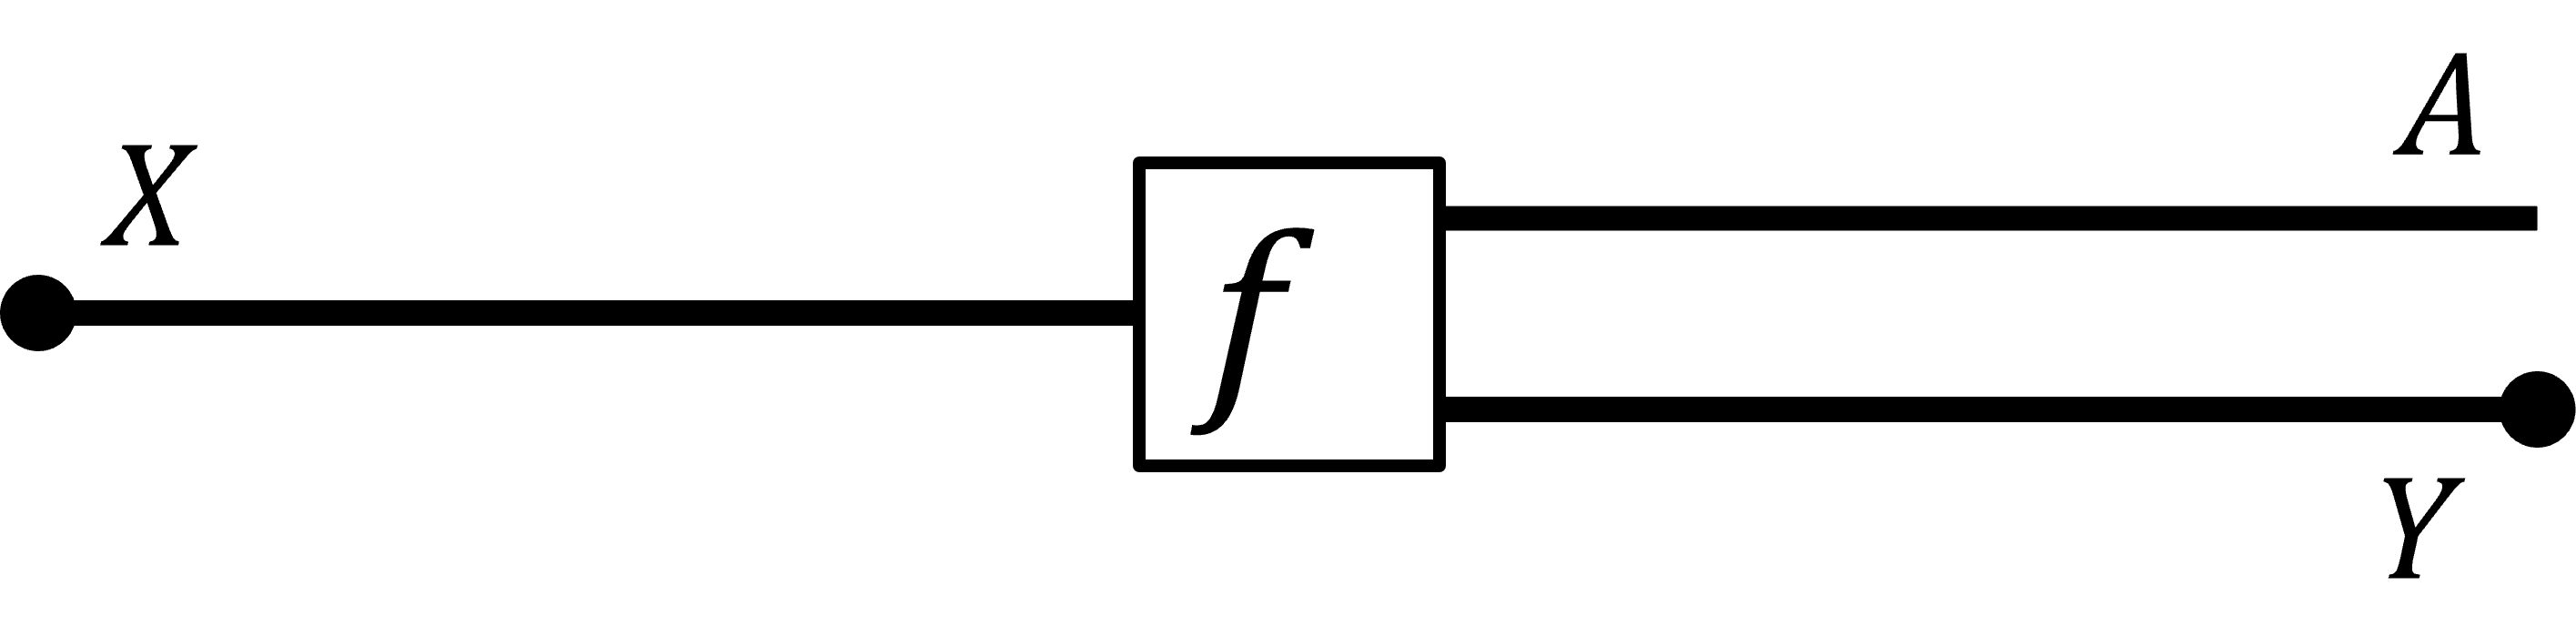
\includegraphics[keepaspectratio, width=8cm]{02_f.png}\\
        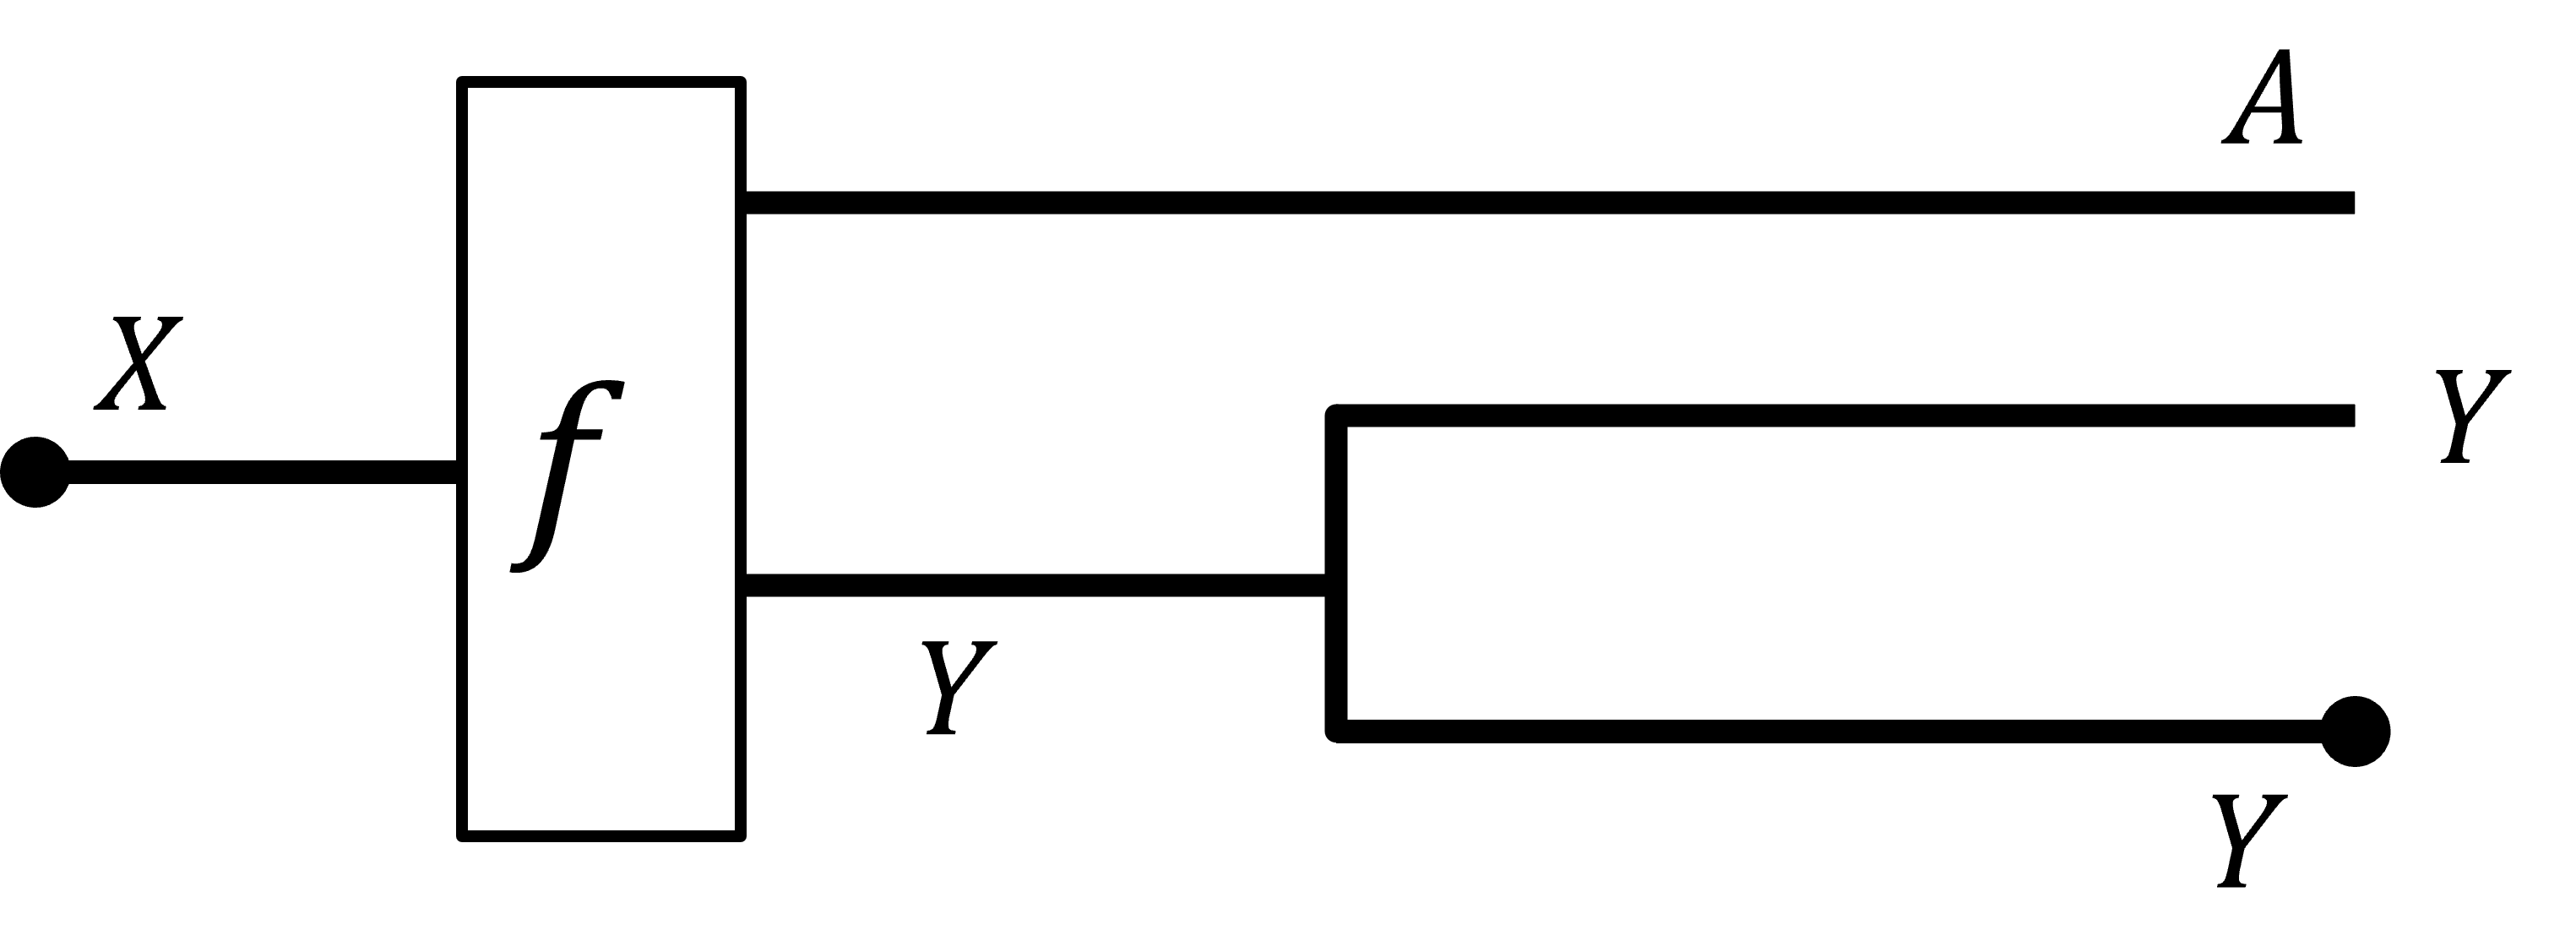
\includegraphics[keepaspectratio, width=8cm]{03_f_comp_a_tens_delta.png}\\
        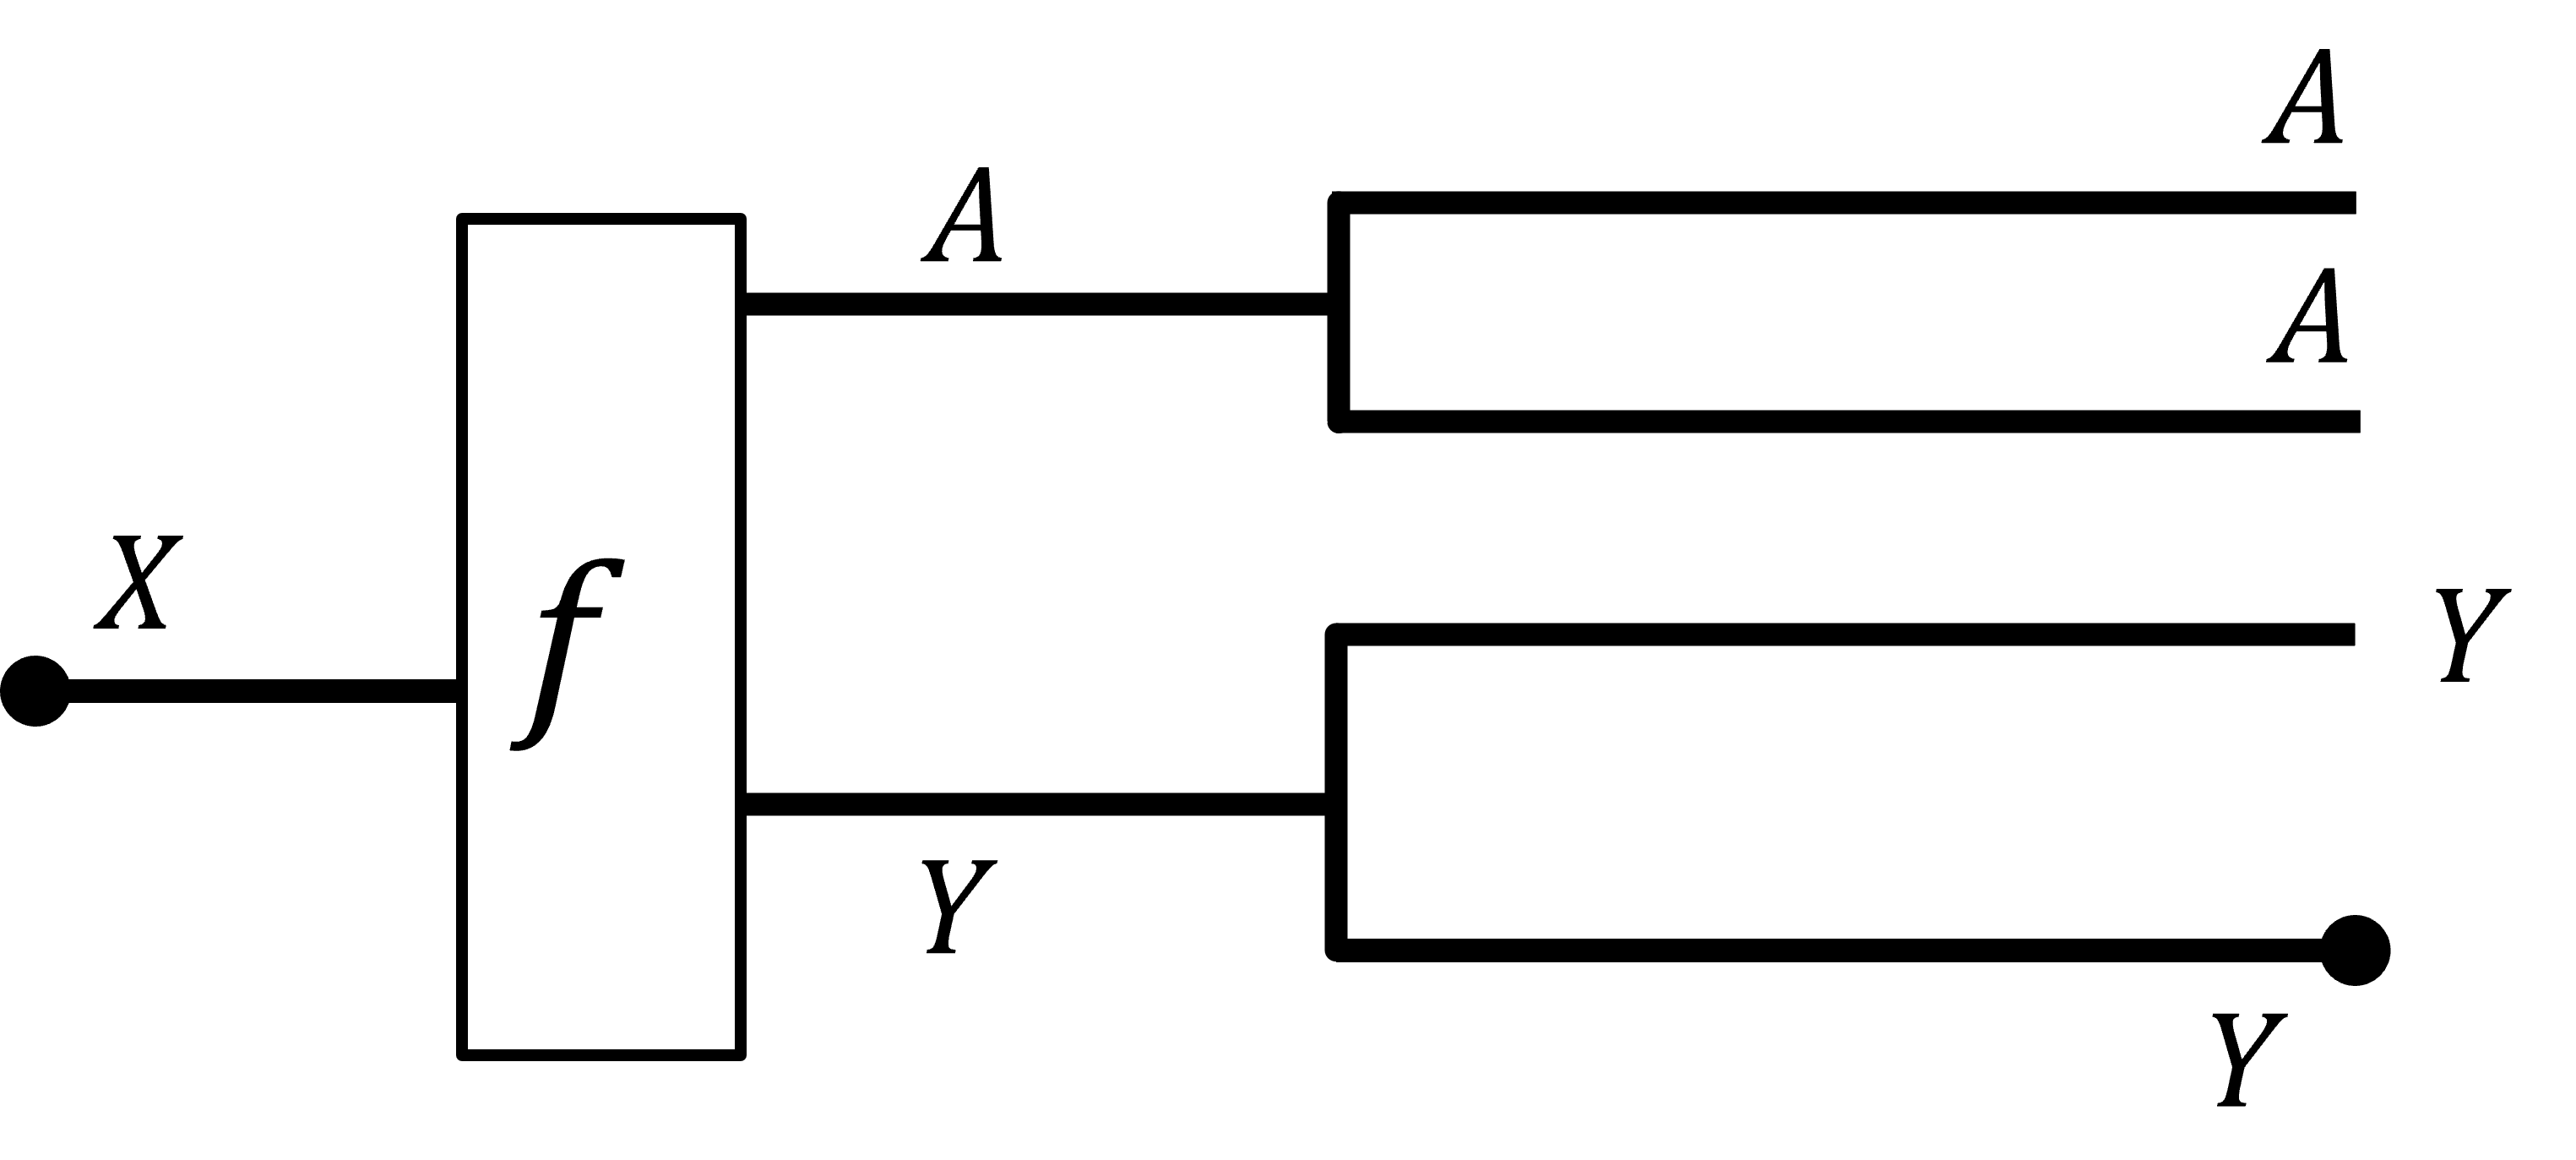
\includegraphics[keepaspectratio, width=8cm]{04_f_comp_delta_tens_delta.png}\\
        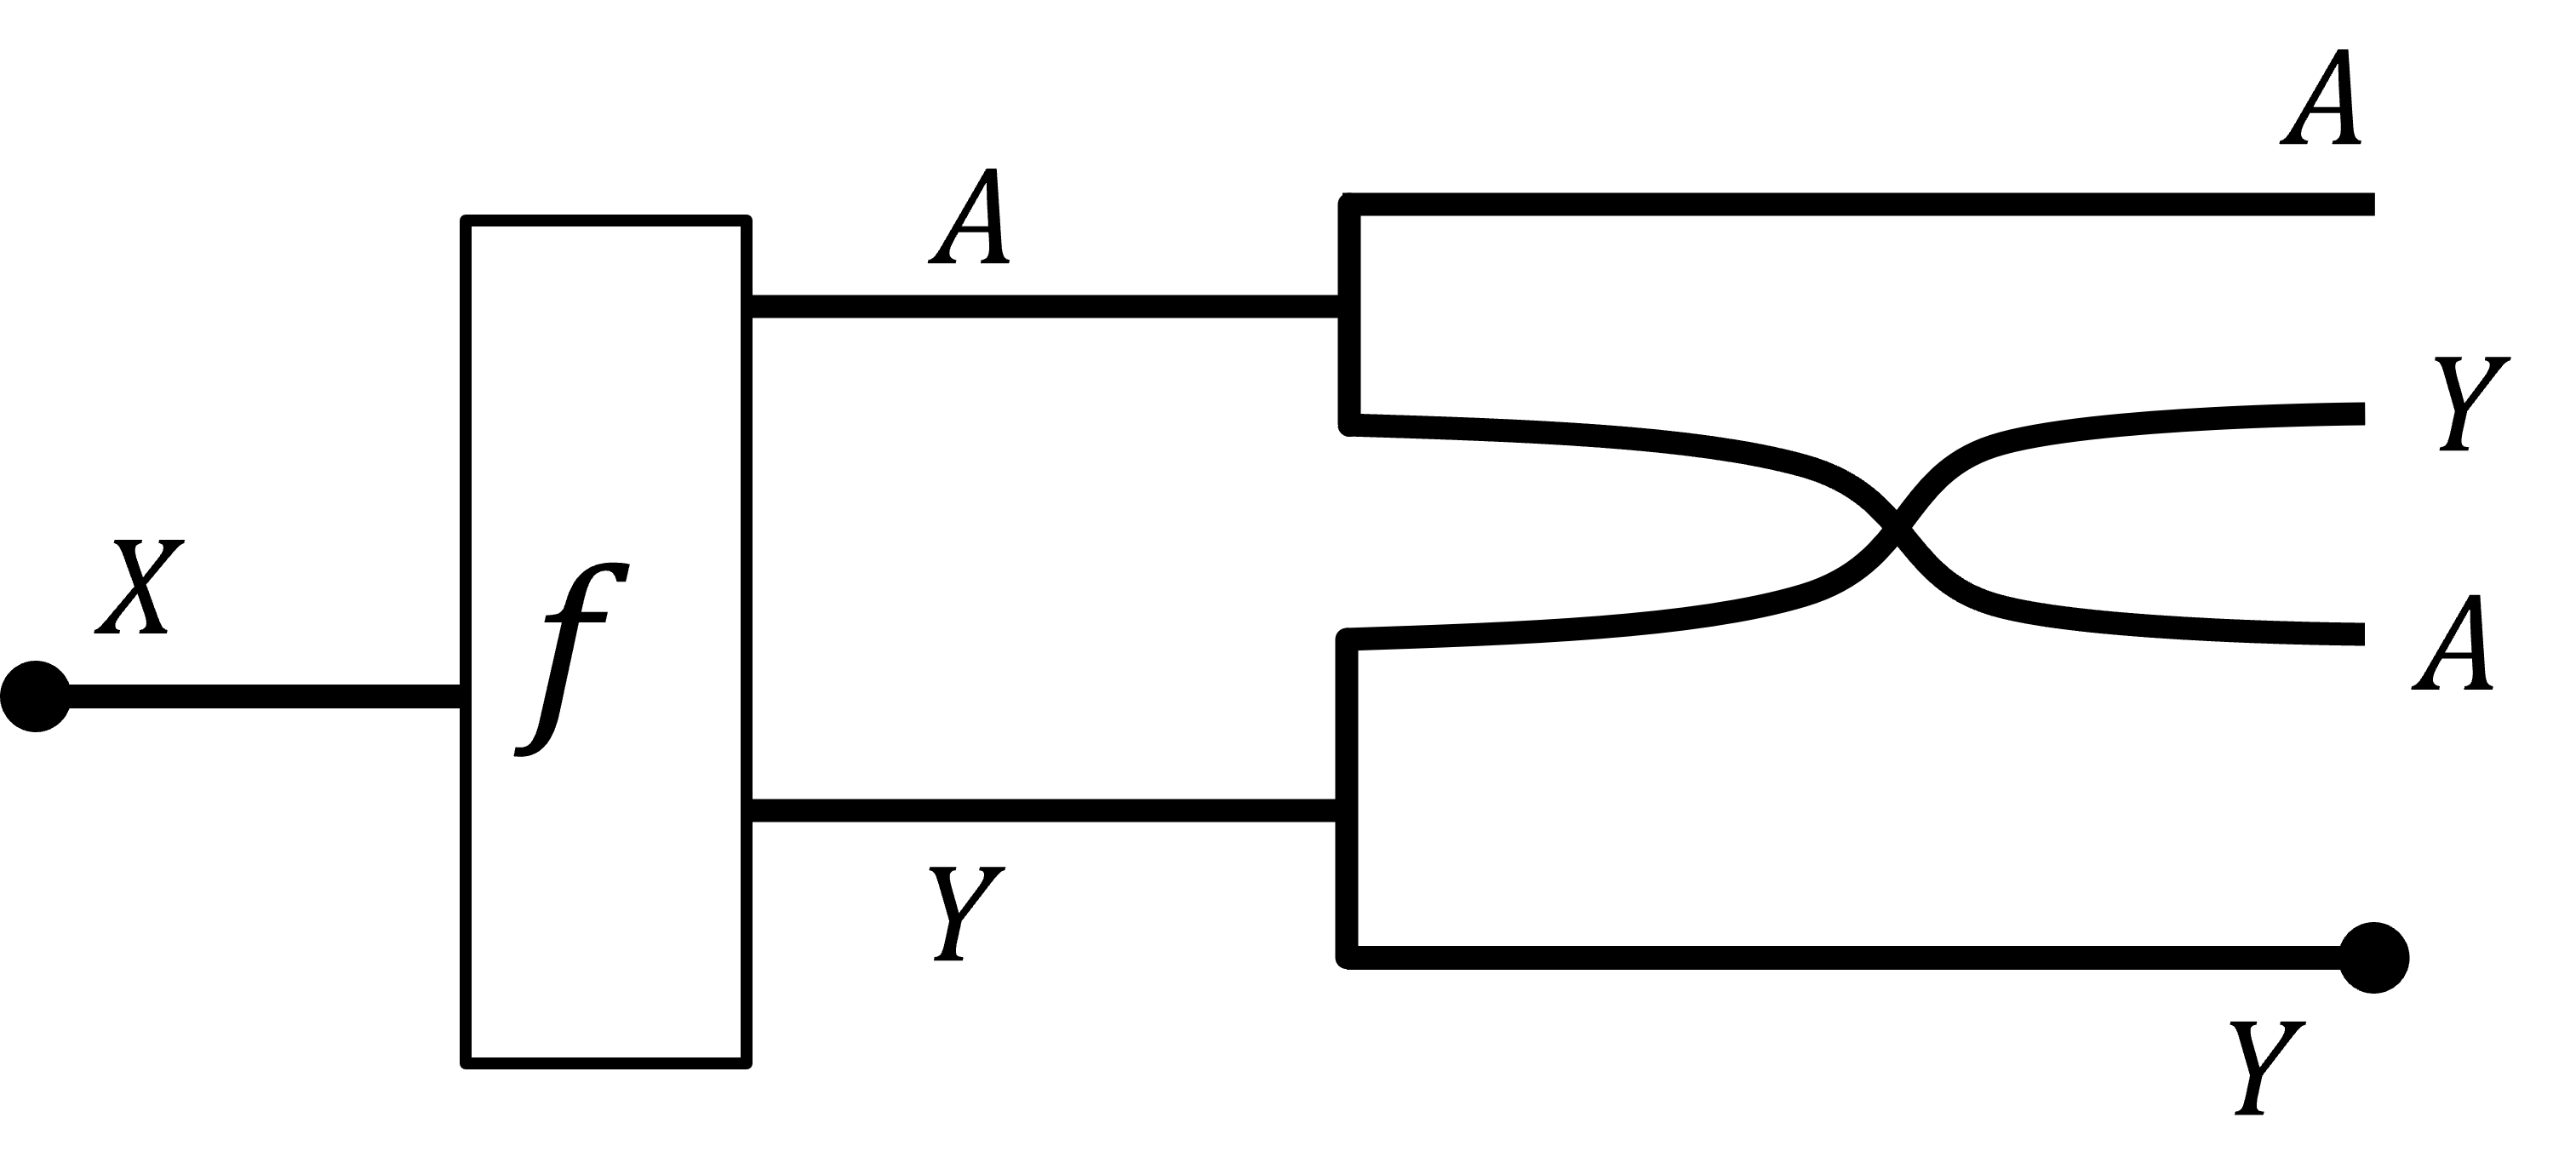
\includegraphics[keepaspectratio, width=8cm]{05_f_comp_delta_tens_delta_comp_gamma.png}\\
        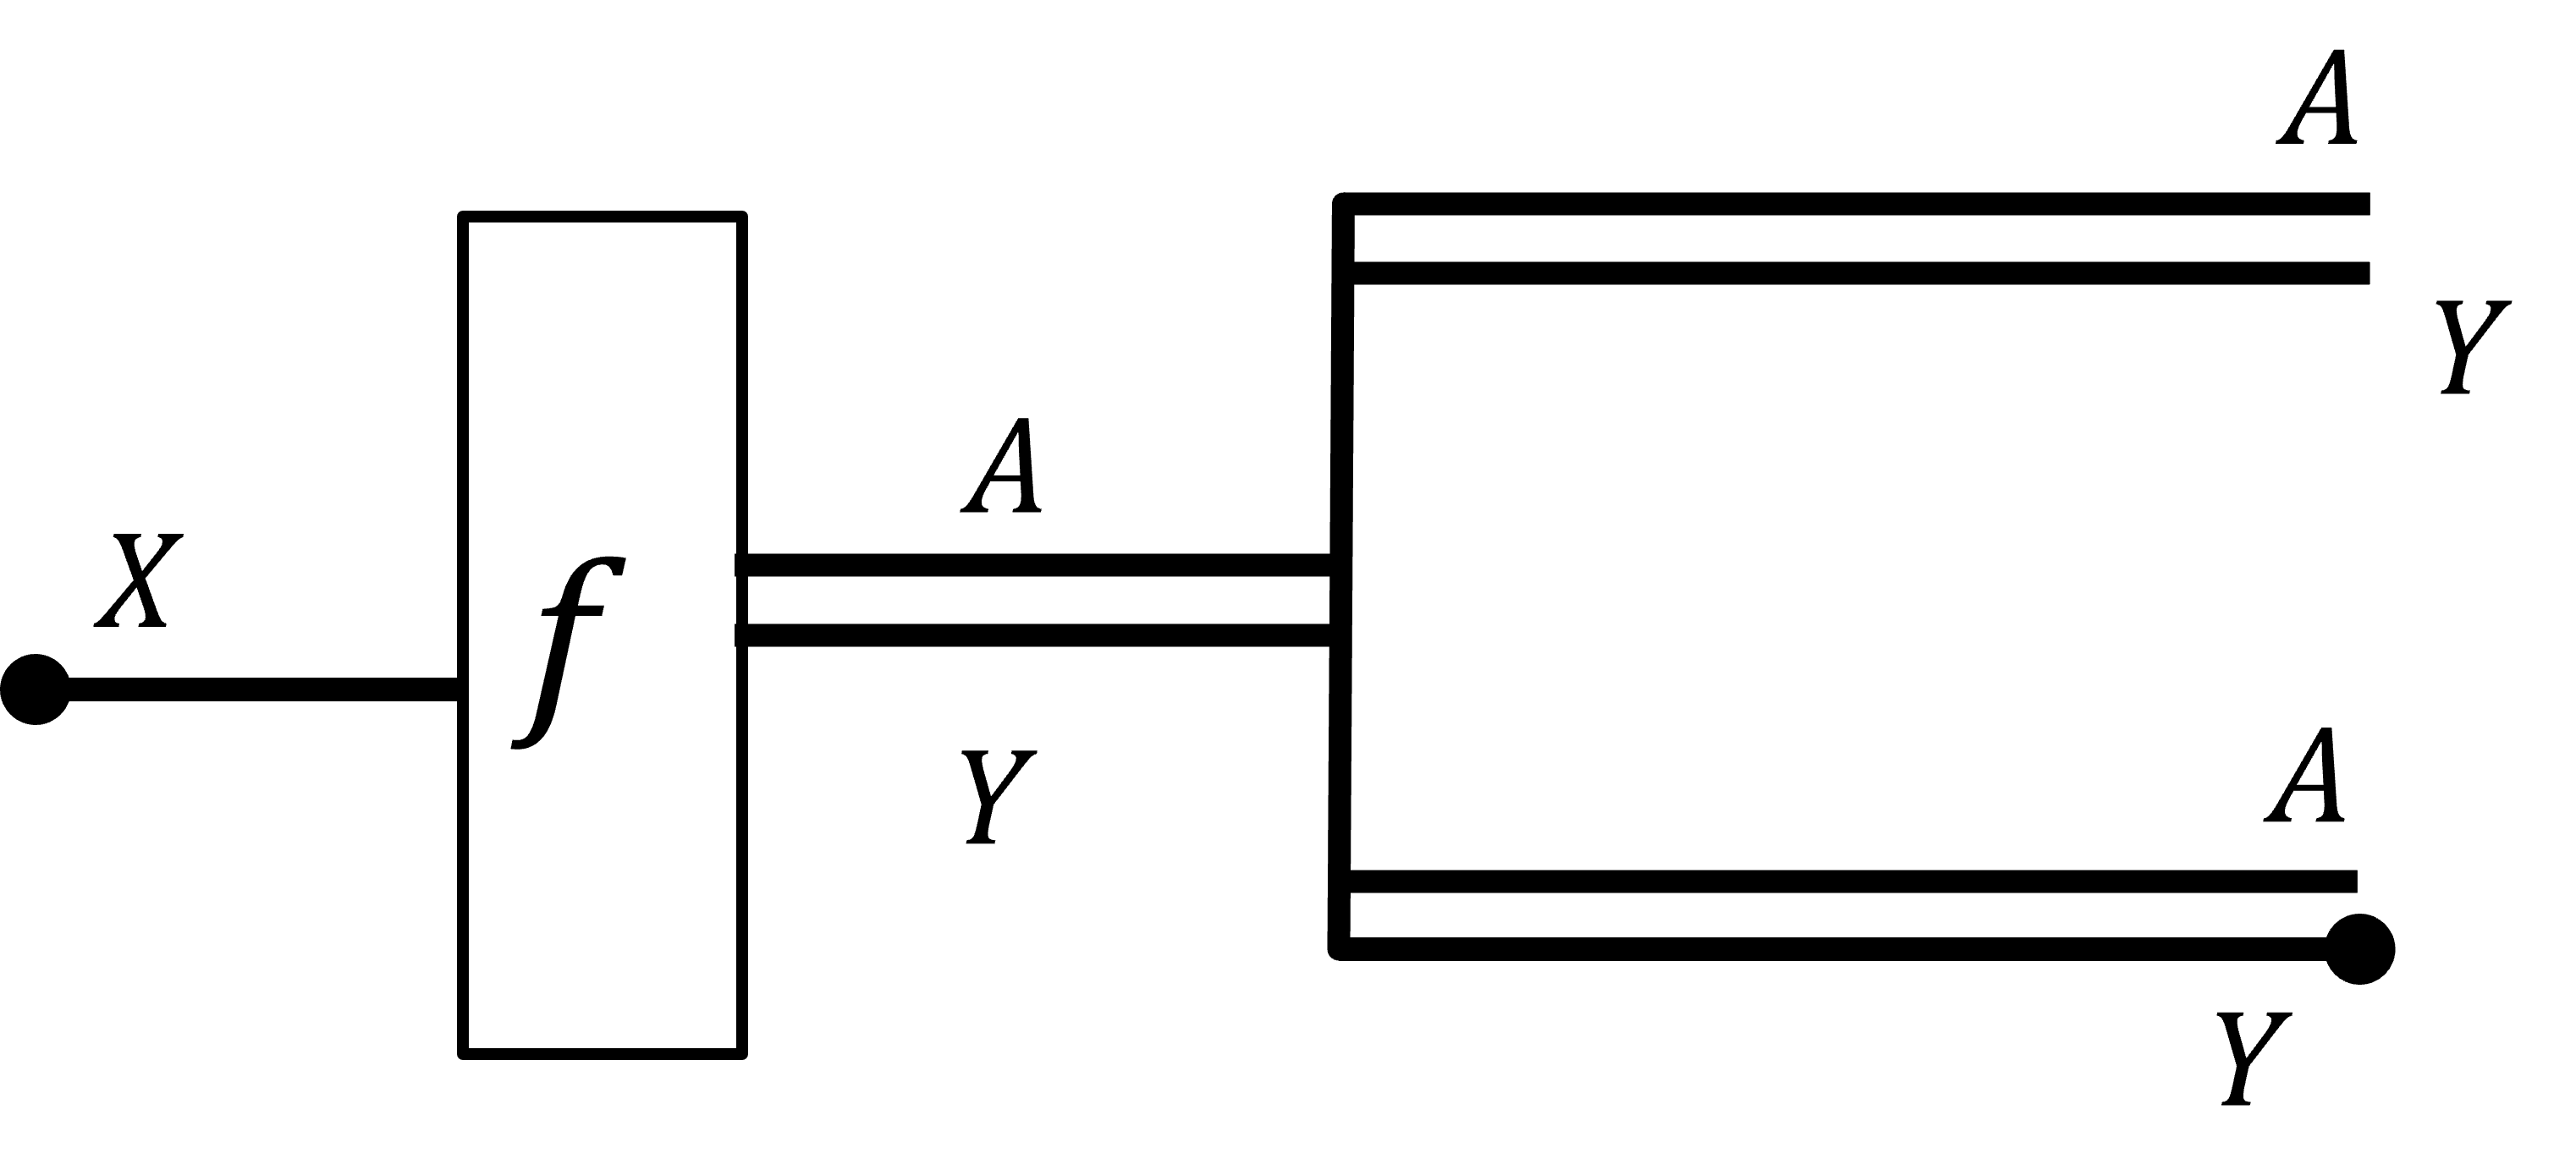
\includegraphics[keepaspectratio, width=8cm]{06_f_comp_delta.png}\\
        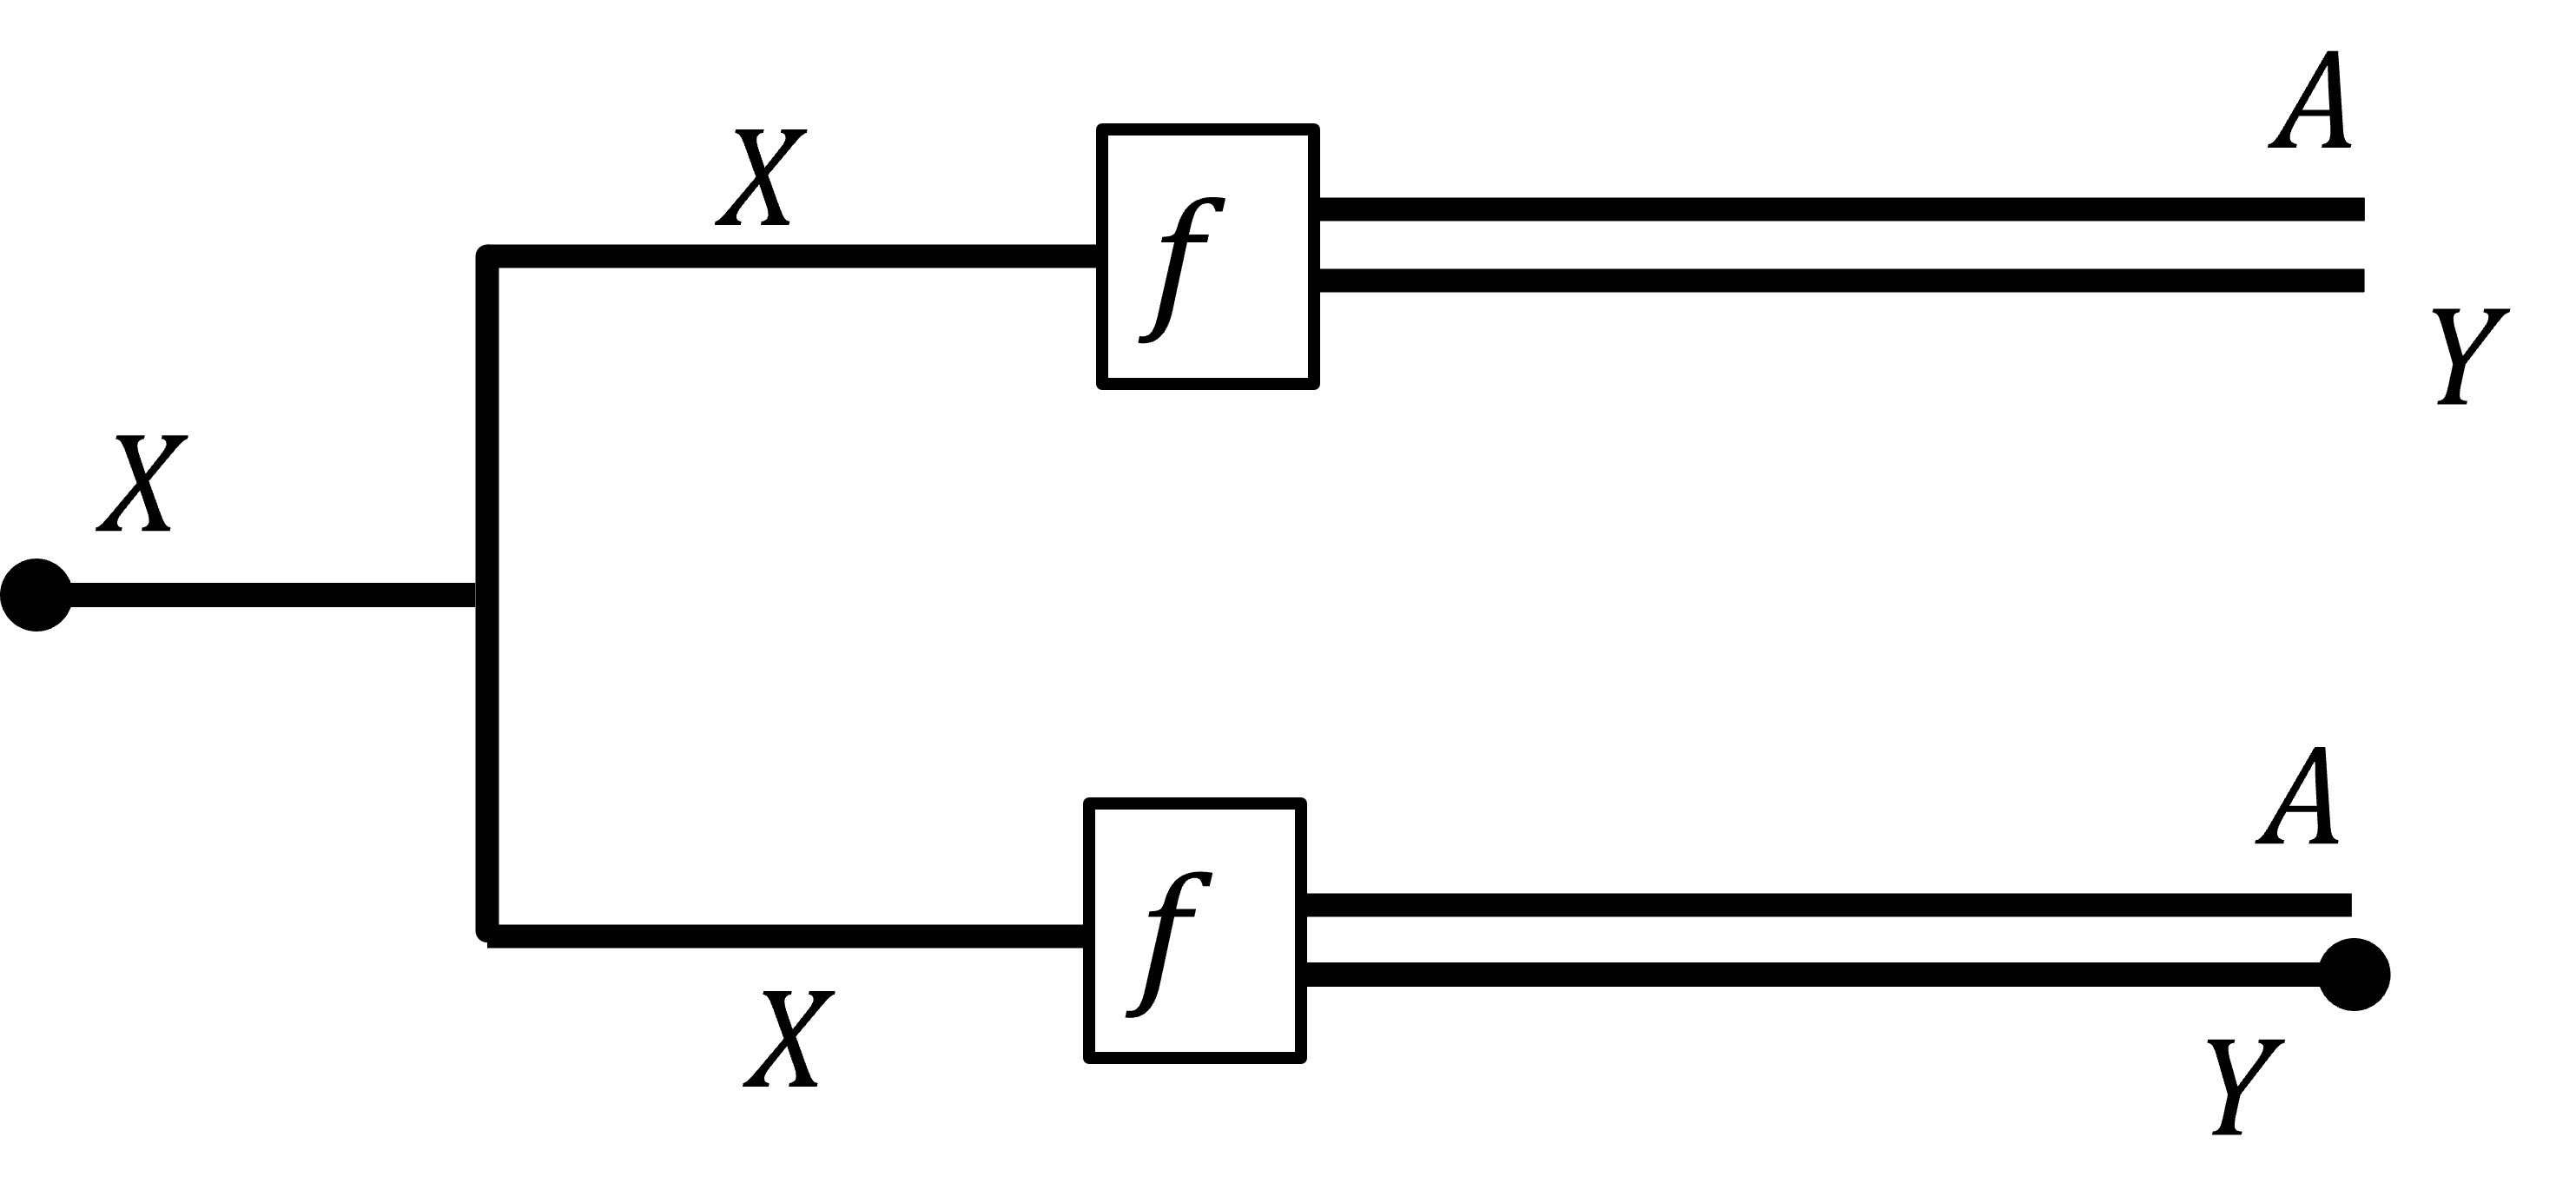
\includegraphics[keepaspectratio, width=8cm]{07_delta_comp_f_tens_f.png}\\
        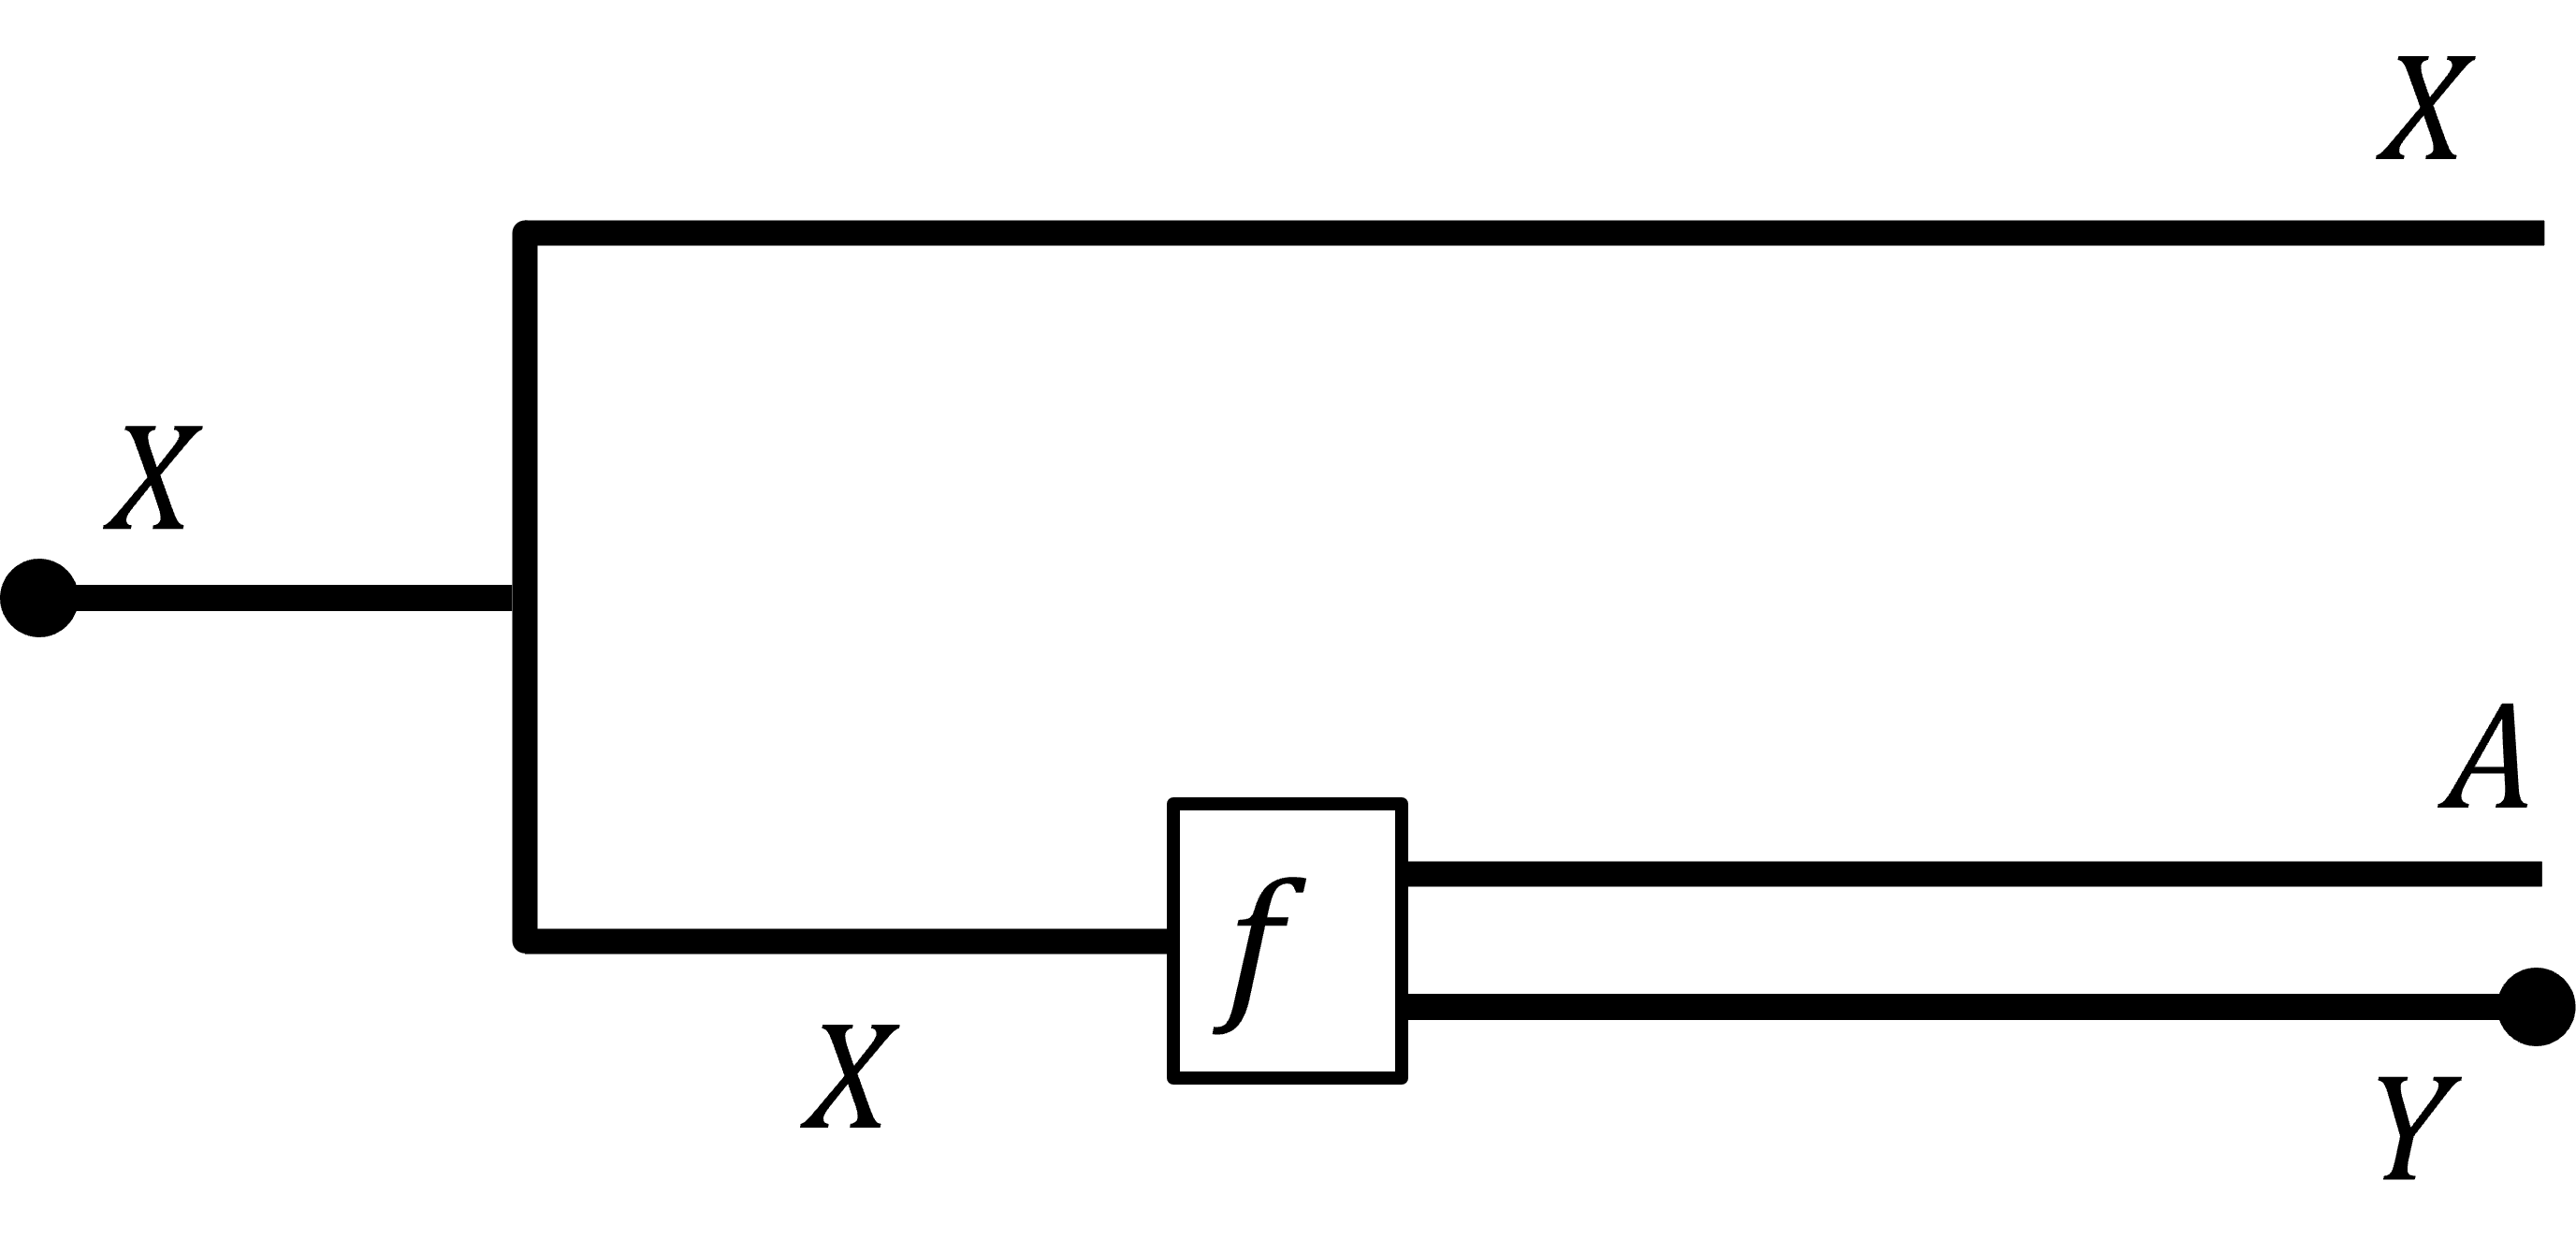
\includegraphics[keepaspectratio, width=8cm]{08_delta_comp_x_tens_f.png}\\
        \caption{String Diagramによる証明}
        \label{fig:my_label}
    \end{figure}
\end{proof}


\paragraph{Lemma \arabic{section}.3.4:\ $\Lambda(\R)$の射の合成のwell-defined性}\ \\
$X,Y,Z\in\calLambda(\R)$とする。
任意の$(A_1,f_1),(A_2,f_2)\in\calLambda(\R)(\bar{X},\bar{Y}),\ (B_1,g_1),(B_2,g_2) \in\calLambda(\R)(\bar{Y},\bar{Z})$に対し、
$(A_1,f_1) \sim (A_2,f_2)$かつ$(B_1,g_1) \sim (B_2,g_2)$ならば、
$(A_1,f_1)\comp(B_1,g_1) \sim (A_2,f_2)\comp(B_2,g_2)$である。

\begin{proof}
    同値関係$\sim$は2-射の生成する同値関係として定義されていたので、次の2つを示せばよい:\\
    (1) 任意の$(A_1,f_1),(A_2,f_2)\in\calLambda(\R)(\bar{X},\bar{Y}), (B,g)\in\calLambda(\R)(\bar{Y},\bar{Z})$
    及び$k:(A_1,f_1)\to (A_2,f_2)$に対し、$(A_1,f_1)\comp(B,g) \sim (A_2,f_2)\comp(B,g)$である。\\
    (2) 任意の$(A,f)\in\calLambda(\R)(\bar{X},\bar{Y}), (B_1,g_1),(B_2,g_2)\in\calLambda(\R)(\bar{Y},\bar{Z})$
    及び$l:(B_1,g_1)\to (B_2,g_2)$に対し、$(A,f)\comp(B_1,g_1) \sim (A,f)\comp(B_2,g_2)$である。
    
    このうち(2)はprop \arabic{section}.2.7そのものである。従って、(1)を示せば十分である。

    (1)を示す。
    $(A_1,f_1),(A_2,f_2)\calLambda(\R)(\bar{X},\bar{Y}), (B,g)\in\calLambda(\R)(\bar{X},\bar{Y})$
    及び$k:(A_1,f_1)\to (A_2,f_2)$を任意に固定する。
    $(A_1,f_1)\comp(B,g)$から$(A_2,f_2)\comp(B,g)$へ至る2-射のジグザグを構成する。\\
    
    
    % https://q.uiver.app/?q=WzAsMyxbMCwwLCJbWCJdLFsxLDAsIkFfMVxcdGVuc29yIFkiXSxbMywwLCJBXzFcXHRlbnNvciBCXFx0ZW5zb3IgWl0iXSxbMCwxLCJmXzEiXSxbMSwyLCJBXzFcXHRlbnNvciBnIl1d
    \[\begin{tikzcd}
    	{(X} & {A_1\tensor Y} && {A_1\tensor B\tensor Z)}
    	\arrow["{f_1}", from=1-1, to=1-2]
    	\arrow["{A_1\tensor g}", from=1-2, to=1-4]
    \end{tikzcd}\]
    
    % https://q.uiver.app/?q=WzAsNSxbMCwxLCJcXHNpbVxcIFtYIl0sWzEsMSwiQV8xXFx0ZW5zb3IgWSJdLFszLDEsIkFfMVxcdGVuc29yIFlcXHRlbnNvciBZIl0sWzUsMSwiQV8xXFx0ZW5zb3IgWVxcdGVuc29yIEJcXHRlbnNvciBaXSJdLFsxLDAsIlxcdGV4dHsoYnkgcHJvcCA0LjIuNywgbGVtIDQuMy4zKX0iXSxbMCwxLCJmXzEiXSxbMSwyLCJBXzFcXHRlbnNvclxcRGVsdGFfWSJdLFsyLDMsIkFfMVlcXHRlbnNvciBnIl1d
    \[\begin{tikzcd}
    	& {\text{(by prop \arabic{section}.2.7, lem \arabic{section}.3.3)}} \\
    	{\sim\ (X} & {A_1\tensor Y} && {A_1\tensor Y\tensor Y} && {A_1\tensor Y\tensor B\tensor Z)}
    	\arrow["{f_1}", from=2-1, to=2-2]
    	\arrow["{A_1\tensor\Delta_Y}", from=2-2, to=2-4]
    	\arrow["{A_1Y\tensor g}", from=2-4, to=2-6]
    \end{tikzcd}\]
    
    % https://q.uiver.app/?q=WzAsNCxbMCwwLCJcXHNpbVxcIFtYIl0sWzEsMCwiQV8xXFx0ZW5zb3IgWSJdLFszLDAsIkFfMVxcdGVuc29yIFlcXHRlbnNvciBZIl0sWzUsMCwiQV8xXFx0ZW5zb3IgWVxcdGVuc29yIEJcXHRlbnNvciBaIl0sWzAsMSwiZl8xIl0sWzEsMiwiQV8xXFx0ZW5zb3JcXERlbHRhX1kiXSxbMiwzLCJBXzFZXFx0ZW5zb3IgZyJdXQ==
    \[\begin{tikzcd}
    	{\sim\ (X} & {A_1\tensor Y} && {A_1\tensor Y\tensor Y} && {A_1\tensor Y\tensor B\tensor Z}
    	\arrow["{f_1}", from=1-1, to=1-2]
    	\arrow["{A_1\tensor\Delta_Y}", from=1-2, to=1-4]
    	\arrow["{A_1Y\tensor g}", from=1-4, to=1-6]
    \end{tikzcd}\]
    
    % https://q.uiver.app/?q=WzAsNCxbMCwwXSxbNCwwLCJBXzJcXHRlbnNvciBZXFx0ZW5zb3IgQlxcdGVuc29yIFpdIl0sWzUsMCwiXFx0ZXh0eyhieSBwcm9wIDQuMi4zLCBwcm9wIDQuMi43KX0iXSxbMiwwXSxbMywxLCJrXFx0ZW5zb3IgQloiXV0=
    \[\begin{tikzcd}
    	{} && {} && {A_2\tensor Y\tensor B\tensor Z)} & {\text{(by prop \arabic{section}.2.3, prop \arabic{section}.2.7)}}
    	\arrow["{k\tensor BZ}", from=1-3, to=1-5]
    \end{tikzcd}\]
    
    % https://q.uiver.app/?q=WzAsNCxbMCwwLCI9XFwgW1giXSxbMSwwLCJBXzFcXHRlbnNvciBZIl0sWzMsMCwiQV8xXFx0ZW5zb3IgWVxcdGVuc29yIFkiXSxbNSwwLCJBXzJcXHRlbnNvciBZXFx0ZW5zb3IgWSJdLFswLDEsImZfMSJdLFsxLDIsIkFfMVxcdGVuc29yXFxEZWx0YV9ZIl0sWzIsMywia1xcdGVuc29yIFkiXV0=
    \[\begin{tikzcd}
    	{=\ (X} & {A_1\tensor Y} && {A_1\tensor Y\tensor Y} && {A_2\tensor Y\tensor Y}
    	\arrow["{f_1}", from=1-1, to=1-2]
    	\arrow["{A_1\tensor\Delta_Y}", from=1-2, to=1-4]
    	\arrow["{k\tensor Y}", from=1-4, to=1-6]
    \end{tikzcd}\]
    
    % https://q.uiver.app/?q=WzAsNCxbMCwwXSxbNCwwLCJBXzJcXHRlbnNvciBZXFx0ZW5zb3IgQlxcdGVuc29yIFpdIl0sWzUsMCwiXFx0ZXh0eyhieSBmdW5jdG9yaWFsaXR5IG9mICRcXHRlbnNvciQpfSJdLFsyLDBdLFszLDEsIkFfMllcXHRlbnNvciBnIl1d
    \[\begin{tikzcd}
    	{} && {} && {A_2\tensor Y\tensor B\tensor Z)} & {\text{(by functoriality of $\tensor$)}}
    	\arrow["{A_2Y\tensor g}", from=1-3, to=1-5]
    \end{tikzcd}\]
    
    % https://q.uiver.app/?q=WzAsNSxbMCwwLCI9XFwgW1giXSxbMSwwLCJBXzJcXHRlbnNvciBZIl0sWzMsMCwiQV8yXFx0ZW5zb3IgWVxcdGVuc29yIFkiXSxbNSwwXSxbNywwXSxbMCwxLCJmXzIiXSxbMSwyLCJBXzJcXHRlbnNvclxcRGVsdGFfWSJdXQ==
    \[\begin{tikzcd}
    	{=\ (X} & {A_2\tensor Y} && {A_2\tensor Y\tensor Y} && {} && {}
    	\arrow["{f_2}", from=1-1, to=1-2]
    	\arrow["{A_2\tensor\Delta_Y}", from=1-2, to=1-4]
    \end{tikzcd}\]
    
    % https://q.uiver.app/?q=WzAsNCxbMCwwXSxbNCwwLCJBXzJcXHRlbnNvciBZXFx0ZW5zb3IgQlxcdGVuc29yIFpdIl0sWzUsMCwiXFx0ZXh0eyhiZWNhdXNlICRrJCBpcyBhIDItbW9ycGhpc20gZnJvbSAkKEFfMSwgZl8xKSQgdG8gJChBXzIsIGZfMikkKX0iXSxbMiwwXSxbMywxLCJBXzJZXFx0ZW5zb3IgZyJdXQ==
    \[\begin{tikzcd}
    	{} && {} && {A_2\tensor Y\tensor B\tensor Z)} & {\text{(because $k$ is a 2-morphism from $(A_1, f_1)$ to $(A_2, f_2)$)}}
    	\arrow["{A_2Y\tensor g}", from=1-3, to=1-5]
    \end{tikzcd}\]
    
    % https://q.uiver.app/?q=WzAsNixbMCwwLCJcXHNpbVxcIFtYIl0sWzEsMCwiQV8yXFx0ZW5zb3IgWSJdLFszLDAsIkFfMlxcdGVuc29yIEJcXHRlbnNvciBaXSJdLFs1LDBdLFs3LDBdLFs0LDAsIlxcdGV4dHsoYnkgcHJvcCA0LjIuNyBhbmQgNC4zLjMpfSJdLFswLDEsImZfMiJdLFsxLDIsIkFfMlxcdGVuc29yIGdfMiJdXQ==
    \[\begin{tikzcd}
    	{\sim\ (X} & {A_2\tensor Y} && {A_2\tensor B\tensor Z)} & {\text{(by prop \arabic{section}.2.7 and \arabic{section}.3.3)}} & {} && {}
    	\arrow["{f_2}", from=1-1, to=1-2]
    	\arrow["{A_2\tensor g_2}", from=1-2, to=1-4]
    \end{tikzcd}\]
    
    以上で示された。
    %(スト図書きてぇ~~~~~~~)
\end{proof}


\paragraph{Definition \arabic{section}.\arabic{subsection}.5:\ $\Lambda(\R)$の射の合成}\ \\
$\bar{X},\bar{Y},\bar{Z}\in\Lambda(\R), [A,f]\in\Lambda(\R)(\bar{X},\bar{Y}), [B,g]\in\Lambda(\R)(\bar{Y},\bar{Z})$とする。
これらの合成を$[A,f]\comp[B,g]:=[(A,f)\comp(B,g)]$で定める。これはlemma\arabic{section}.3.4よりwell-definedである。

\paragraph{Definition \arabic{section}.\arabic{subsection}.6:\ $\Lambda(\R)$の恒等射}\ \\
各$\bar{X}\in\Lambda(\R)$に対し、$id_{\bar{X}}:=[I,\rho_X^{-1}]$と定める。

\paragraph{Proposition \arabic{section}.\arabic{subsection}.7:\ $\Lambda(\R)$の結合則}\ \\
上記compositionは結合則を満たす。
これは$\calLambda(\R)$で1-射の結合則が成り立っていたことから従う。

\paragraph{Proposition \arabic{section}.\arabic{subsection}.8:\ $\Lambda(\R)$の単位律}\ \\
上記合成とidentityは単位律を満たす。

\paragraph{Definition \arabic{section}.\arabic{subsection}.9:\ 圏 $\Lambda(\R)$}\ \\
definition \arabic{section}.3.1, \arabic{section}.3.2, \arabic{section}.3.5, \arabic{section}.3.6 で与えられる構造達は、
proposition\arabic{section}.3.7, \arabic{section}.3.8より、圏を成す。
この圏を$\Lambda(\R)$と書くことにする。\\


\newpage
\subsection{Cartesian Structure of the Category \texorpdfstring{$\Lambda(\R)$}{Lambda(R)}}
以上で定義した$\Lambda(\R)$が\CC になっていることを示す。
実は$\R$から引き継ぐモノイド構造がそのまま直積となる。
まずモノイド構造を引き継ぐことを示し、その後それが直積の普遍性を持つことを示す。
%the category $\Lambda(\R)$ defined in previous sections, becomes cartesian category. In this section, we will find its cartesian structure and prove that.


\paragraph{Definition \arabic{section}.4.1:\texorpdfstring{$\Lambda(\R)$}{Lambda(R)}のモノイド構造}\ \\
$\R$を \RC とする。
$\Lambda(\R)$は、素朴な方法で\SMC となる。
モノイド積の函手$\tensor'$のみ明示する。$\tensor'$を次のように定める。
\fct{\tensor'}{\Lambda(\R)\times \Lambda(\R)}{\Lambda(\R)}{(X,Y)}{([A,f], [B,g])}{(X',Y')}{X\tensor Y}{[A\tensor B, f\square g]}{X'\tensor Y'}
ただし、$f\square g := (f\tensor g)\comp (A\tensor\gamma_{X,B}\tensor Y)$ である。
このように定めた$\tensor'$は確かにwell-definedである。
%次に単位対象を $I':=I$で定める。
%整合性の同型$\alpha', \lambda', \rho'$及び捻り同型$\gamma'$を素朴な方法で定めると、$(\Lambda(\R),\tensor')$

%$\Delta$の構成


\paragraph{Proposition \arabic{section}.4.3:$\Lambda[\R]$の直積 }\ \\
簡単のため$\C:=\Lambda[\R]$とおく。
$X,Y\in\C$に対し、$(X\tensor Y, \pi_X, \pi_Y)$は$X$と$Y$の直積である。
ただし、$\pi_Y:X\tensor Y\to Y$は、$\pi_Y:=[X,id_{X\tensor Y}]$で定める。
$\pi_X:X\tensor Y\to X$は、$\pi_X:=[Y,\gamma_{X,Y}]$で定める。

\begin{proof}
    $Z\in\C$を任意に取る。
    対応
    $\phi:\C(Z,X\tensor Y)\to \C(Z,X)\times\C(Z,Y)$を
    $\phi([C,h]):=([C,h]\comp\pi_X, [C,h]\comp\pi_Y)$で定める。
    $\phi$が全単射であることを示す。

    次の3つのことをすればよい。\\
    (i)\ $\phi$の逆対応$\psi$を構成する。\\
    (ii)\ $\psi\comp\phi=id$であることを示す。\\
    (iii)\ $\phi\comp\psi=id$であることを示す。\\
    
    \noindent
    (i)\ $\phi$の逆対応$\psi$を構成する。
    
    $[A,f]:Z\to X, \ [B,g]:Z\to Y$を任意に取る。
    $\R$の射 $f\boxdot g$を$f\boxdot g :=\Delta_{Z}\comp (f\square g)$で定める。
    即ち$f\boxdot g$は次の列の合成である:
    \[
    Z\to Z\tensor Z\to(A\tensor X)\tensor(B\tensor Y)\to(A\tensor B)\tensor(X\tensor Y)
    \]
    %$\underline{Z}\to\underline{Z}\tensor\underline{Z}\to(A\tensor\underline{X})\tensor(B\tensor\underline{Y})\to(A\tensor B)\tensor(\underline{X}\tensor\underline{Y})$
    $\psi([A,f],[B,g]):=[A\tensor B, f\boxdot g]$とする。
    $\psi$のwell-defined性を示す。次の2つを示せばよい:\\
    (a)\ 任意の$(A_1,f_1),(A_2,f_2):Z\to X, (B,g):Z\to Y \rmin \calLambda(\R)$と$k:(A_1,f_1)\to(A_2,f_2)$に対し、$(A_1\tensor B, f_1\boxdot g)\sim (A_2\tensor B, f_2\boxdot g)$である。\\
    (b)\ 任意の$(A,f):Z\to X, (B_1,g_1),(B_2,g_2):Z\to Y \rmin \calLambda(\R)$と$l:(B_1,g_1)\to(B_2,g_2)$に対し、$(A\tensor B_1, f\boxdot g_1)\sim (A\tensor B_2, f\boxdot g_2)$である。
    
    両者の証明は同様なので(a)のみ示す。
    $k\tensor BXY:(A_1\tensor B, f_1\boxdot g)\to (A_2\tensor B, f_2\boxdot g)$は次の図式を可換にするから、確かに$(A_1\tensor B, f_1\boxdot g)$から$(A_2\tensor B, f_2\boxdot g)$への2-射である。
    % https://q.uiver.app/?q=WzAsNSxbMiwwLCJBXzFcXHRlbnNvciBCXFx0ZW5zb3IgWFxcdGVuc29yIFkiXSxbMCwxLCJaIl0sWzIsMiwiQV8yXFx0ZW5zb3IgQlxcdGVuc29yIFhcXHRlbnNvciBZIl0sWzQsMCwiQV8xXFx0ZW5zb3IgQlxcdGVuc29yIFhcXHRlbnNvciBZXFx0ZW5zb3IgWFxcdGVuc29yIFkiXSxbNCwyLCJBXzFcXHRlbnNvciBCXFx0ZW5zb3IgWFxcdGVuc29yIFlcXHRlbnNvciBYXFx0ZW5zb3IgWSJdLFsxLDAsImZfMVxcYm94ZG90IGciXSxbMCwyLCJrXFx0ZW5zb3IgQlhZIl0sWzEsMiwiZl8yXFxib3hkb3QgZyIsMl0sWzAsMywiXFxEZWx0YSJdLFszLDQsImtcXHRlbnNvciBCWFlYWSJdLFsyLDQsIlxcRGVsdGEiXV0=
    \[\begin{tikzcd}
    	&& {A_1\tensor B\tensor X\tensor Y} && {A_1\tensor B\tensor X\tensor Y\tensor X\tensor Y} \\
    	Z \\
    	&& {A_2\tensor B\tensor X\tensor Y} && {A_1\tensor B\tensor X\tensor Y\tensor X\tensor Y}
    	\arrow["{f_1\boxdot g}", from=2-1, to=1-3]
    	\arrow["{k\tensor BXY}", from=1-3, to=3-3]
    	\arrow["{f_2\boxdot g}"', from=2-1, to=3-3]
    	\arrow["\Delta", from=1-3, to=1-5]
    	\arrow["{k\tensor BXYXY}", from=1-5, to=3-5]
    	\arrow["\Delta", from=3-3, to=3-5]
    \end{tikzcd}\]

    \noindent
    (ii)$\psi\comp\phi=id$であることを示す。
    $[A,f]:Z\to X, \ [B,g]:Z\to Y$を任意に取る。
    $([A\tensor B, f\boxdot g]\comp \pi_X,\ [A\tensor B, f\boxdot g]\comp \pi_Y) = ([A,f], [B,g])$
    であることを示す。
    $([A\tensor B, f\boxdot g]\comp \pi_Y) = [B,g]$
    であることのみ示す。
    \begin{align*}
        [A\tensor B, f\boxdot g]\comp \pi_Y = &\ [A\tensor B\tensor X, f\boxdot g]\ \ \ (\text{by def of}\ \ \comp \ )\\
        = &\ [A\tensor B\tensor X,\Delta_Z\comp(f\tensor g) \comp(A\tensor\gamma_{X,B}\tensor Y)]\ \ \ 
        (\text{by def of}\ \boxdot \ )\\
        = &\ [A\tensor X\tensor B, \Delta_Z \comp (f\tensor g)]\ \ \  
        (\text{by prop \arabic{section}.2.3})\\
        = &\ [Z\tensor B, \Delta_Z \comp (Z\tensor g)]\ \ \  
        (\text{by prop \arabic{section}.2.3})\\
        = &\ [B,g]\ \ \  
        (\text{by prop \arabic{section}.3.3})
    \end{align*}
    $([A\tensor B, f\boxdot g]\comp \pi_X) = [A,f]$
    であることの証明も同様である。
    以上で$\psi\comp\phi=id$であることが示された。\\
    %$[C,h]:Z\to X\tensor Y$であって次の図式(*)を満たすものを構成する。\\

    \noindent
    (iii)$\phi\comp\psi=id$であることを示す。
    $[C,h]:Z\to X\tensor Y$を任意に取る。
    $[C,h]=\psi(\phi([C,h]))$であることを示す。
    \begin{align*}
        &\psi(\phi([C,h]))\\
        = &\ \psi([C,h]\comp\pi_X, [C,h]\comp\pi_Y)\ \ \ 
        (\text{by def of}\ \ \phi \ )\\
        = &\ \psi([C\tensor Y,h\comp(C\tensor\gamma_{X,Y})], [C\tensor X,h])\ \ \ 
        (\text{by def of}\ \ \comp \ )\\
        = &\ [C\tensor Y\tensor C\tensor X, \ (h\comp(C\tensor\gamma_{X,Y}))\boxdot h]\ \ \  
        (\text{by def of}\ \psi \ )\\
        = &\ [C\tensor Y\tensor C\tensor X,\  \Delta_Z\comp((h\comp(C\tensor\gamma_{X,Y}))\tensor h) \comp(CY\tensor\gamma_{X,CX}\tensor Y)]\ \ \  
        (\text{by def of}\ \boxdot )\\
        = &\ [C\tensor Y\tensor C\tensor X,\  \Delta_Z\comp(h\tensor h) 
        \comp(C\tensor\gamma_{X,Y}\tensor CXY)
        \comp(CY\tensor\gamma_{X,CX}\tensor Y)]\ \ \  
        (\text{by functoriality of}\ \tensor)\\
        = &\ [C\tensor Y\tensor C\tensor X,\  h\comp\Delta_{CXY}
        \comp(C\tensor\gamma_{X,Y}\tensor CXY)
        \comp(CY\tensor\gamma_{X,CX}\tensor Y)]\ \ \ 
        (\text{by naturality of}\ \Delta)\\
        = &\ [C\tensor Y\tensor C\tensor X,\  h
        \comp(\Delta_{C}\tensor\Delta_{XY})
        \comp(C\tensor\gamma_{CX,Y}\tensor XY)]\ \ \ 
        (*)\\
        = &\ [C\tensor C\tensor X\tensor Y,\  h\comp(\Delta_C\tensor\Delta_{XY})]\ \ \ 
        (\text{by prop \arabic{section}.2.3})\\
        = &\ [C\tensor X\tensor Y,\  h\comp(C\tensor\Delta_{XY})]\ \ \ 
        (\text{by prop \arabic{section}.2.3})\\
        = &\ [C,\  h]\ \ \ 
        (\text{by prop \arabic{section}.2.4 and prop \arabic{section}.2.7})
    \end{align*}

    上式中の$(*)$の部分は下のように示される。
    \begin{align*}
        &\ \Delta_{CXY}
        \comp(C\tensor\gamma_{X,Y}\tensor CXY)
        \comp(CY\tensor\gamma_{X,CX}\tensor Y)\\
        = &\ (\Delta_{C}\tensor\Delta_{XY})
        \comp(C\tensor\gamma_{C,XY}\tensor XY)
        \comp(C\tensor\gamma_{X,Y}\tensor CXY)
        \comp(CY\tensor\gamma_{X,CX}\tensor Y)\ \ \ 
        (\text{by monoidality of\ $\Delta$})\\
        = &\ (\Delta_{C}\tensor\Delta_{X}\tensor\Delta_{Y})
        \comp(CCX\tensor\gamma_{X,Y}\tensor Y)
        \comp(C\tensor\gamma_{C,XY}\tensor XY)
        \comp(C\tensor\gamma_{X,Y}\tensor CXY)
        \comp(CY\tensor\gamma_{X,CX}\tensor Y)\ \ \ 
        (\text{by monoidality of\ $\Delta$})\\
        = &\ (\Delta_{C}\tensor\Delta_{X}\tensor\Delta_{Y})
        \comp(CCX\tensor\gamma_{X,Y}\tensor Y)
        \comp(CC\tensor\gamma_{X,Y}\tensor XY)
        \comp(C\tensor\gamma_{C,YX}\tensor XY)
        \comp(CY\tensor\gamma_{X,CX}\tensor Y)\ \ \
        (\text{by coherence})\\
        = &\ (\Delta_{C}\tensor\Delta_{X}\tensor\Delta_{Y})
        \comp(CCX\tensor\gamma_{X,Y}\tensor Y)
        \comp(CC\tensor\gamma_{X,Y}\tensor XY)
        \comp(C\tensor\gamma_{C,Y}\tensor XY)
        \comp(CY\tensor\gamma_{X,X}\tensor Y)\ \ \
        (\text{by coherence})\\
        = &\ (\Delta_{C}\tensor\Delta_{X}\tensor\Delta_{Y})
        \comp(C\tensor\gamma_{CXX,Y}\tensor Y)
        \comp(CY\tensor\gamma_{X,X}\tensor CY)\ \ \
        (\text{by coherence})\\
        = &\ (\Delta_{C}\tensor\Delta_{X}\tensor\Delta_{Y})
        \comp(CC\tensor\gamma_{X,X}\tensor YY)
        \comp(C\tensor\gamma_{CXX,Y}\tensor Y)\ \ \ 
        (\text{by coherence})\\
        = &\ (\Delta_{C}\tensor\Delta_{X}\tensor\Delta_{Y})\ \ \ \ 
        \comp(C\tensor\gamma_{CXX,Y}\tensor Y)\ \ \ 
        (\text{by commutativity of}\ \Delta_X)\\
        = &\ (\Delta_{C}\tensor\Delta_{X}\tensor\Delta_{Y})
        \comp(CCX\tensor\gamma_{X,Y}\tensor Y)
        \comp(C\tensor\gamma_{CX,Y}\tensor XY)\ \ \ 
        (\text{by coherence})\\
        = &\ (\Delta_{C}\tensor\Delta_{XY})
        \comp(C\tensor\gamma_{CX,Y}\tensor XY)]\ \ \ 
        (\text{by monoidality of}\ \Delta)
    \end{align*}
    上式中の(by coherence)と書かれた部分は六角形公理及び函手性・自然性のみから導かれる主張である。
    
    以上で示された。
\end{proof}










\newpage



\section{universality of \texorpdfstring{$\Lambda$}{Lambda} construction}
前節で定義した構成$\Lambda$は、実は関連圏からデカルト圏を得る普遍的な方法になっている。今節ではこの普遍性を示す。
まず$\R$から$\Lambda(\R)$への素朴な埋め込みを定める。

\paragraph{Definition \arabic{section}.1:ユニット函手 $\Eta_{\R}$}\ \\
函手 $\Eta_{\R}:\R\to\Lambda[\R]$を次で定める:
\fct{\Eta_{\R}}{\R}{\Lambda(\R)}{X}{f}{Y}{X}{[I,f\comp\rho_Y]}{Y}
$\Eta_{\R}$は\Rf である。

そして$\Lambda$は次の普遍性を満たす(煩雑な議論を避けるため、2圏論的主張を1圏論的主張に弱めている)。
\paragraph{proposition \arabic{section}.2:\ universality of $\Lambda$}\ \\
$\R$を\RC とし、
\CC \ $\C:=\Lambda[\R]$及び\Rf $\Eta_{\R}:\R \to \C$を上で定めたものとする。\\
このとき、任意の\CC \ $\D$ 及びstrong relevance functor $F=(F,\theta):\R \to \D$に対し、\\
次を満たすstrong cartesian functor $\bar{F}:\C\to\D$が一意に存在する:

$F = \Eta_{\R}\comp \bar{F}$

\begin{proof}
    (i)strong relevance functor $F:\R \to \D$に対しstrong cartesian functor $\bar{F}:\C\to\D$を対応させる操作$\bar{(-)}$を次で定める:\\
    各$\bar{X}\in\C$に対し、$\bar{F}(\bar{X}):=F(X)$.\\
    各$[A,f]:\bar{X}\to \bar{Y}\ \text{in}\ \C$に対し、$\bar{F}([A,f])$を
    $\bar{F}([A,f]):=F(f)\comp\theta_{A,Y}$で定める。\\
    ただし、$\theta_{A,Y}:F(A\tensor Y)\to F(A)\times F(Y)$はFのモノイド函手としての構造の同型である。\\
    分かりやすさのために追記する。これは下の列の合成のことである:\\
    $F(X)\to F(A\tensor Y)\simeq F(A)\times F(Y)\to F(Y)$.\\

    この$\bar{F}$のwell-definednessは以下のようによい:\\
    $(A,f),(B,g):X\to Y \rmin \calLambda(\R)$と$k:(A,f)\to (B,g)$を任意に取る。$\bar{F}$はrelevance functorであったから、次の図式は可換:

    \[
    \adjustbox{scale=0.7, center}{
    \begin{tikzcd}
        &&& {F(A\tensor Y\tensor Y)} && {F(A\tensor Y)\times F(Y)} && {F(A)\times F(Y)\times F(Y)} \\
        && {F(A\tensor Y)} &&&& {F(A)\times F(Y)} \\
        {F(X)} &&& {F(B\tensor Y\tensor Y)} && {F(B\tensor Y)\times F(Y)} && {F(B)\times F(Y)\times F(Y)} && {F(Y)} \\
        && {F(B\tensor Y)} &&&& {F(B)\times F(Y)}
        \arrow["{F(f)}", from=3-1, to=2-3, crossing over]
        \arrow["{F(g)}"', from=3-1, to=4-3, crossing over]
        \arrow["{F(k)}", from=2-3, to=4-3, crossing over]
        \arrow["\Delta", from=2-3, to=1-4, crossing over]
        \arrow["\simeq", from=1-4, to=1-6, crossing over]
        \arrow["\Delta", from=4-3, to=3-4, crossing over]
        \arrow["{F(k\tensor Y)}"{pos=0.3}, from=1-4, to=3-4, crossing over]
        \arrow["\simeq", from=3-4, to=3-6, crossing over]
        \arrow["{F(k)\times F(Y)}"{pos=0.3}, from=1-6, to=3-6, crossing over]
        \arrow["\simeq", from=2-3, to=2-7, crossing over]
        \arrow["\simeq", from=4-3, to=4-7, crossing over]
        \arrow["\simeq", from=1-6, to=1-8, crossing over]
        \arrow["\simeq", from=3-6, to=3-8, crossing over]
        \arrow["\pi"{description}, from=2-7, to=3-10, crossing over]
        \arrow["\pi"{description}, from=4-7, to=3-10, crossing over]
        \arrow[from=2-7, to=1-8, crossing over]
        \arrow[from=4-7, to=3-8, crossing over]
        \arrow["\pi"{description}, from=1-8, to=3-10, crossing over]
        \arrow["\pi"{description}, from=3-8, to=3-10]
    \end{tikzcd}
    }
    \]
    これは確かにCartesian functorである。\\
    %ほぼ自明なので特に説明しない


    (ii)操作 $\bar{(-)}$と $\Eta_{\R}\comp-$が互いに逆であることを示す。\\
    どちらも対象上何も操作しないので、対象の対応が等しいことは直ちに分かる。よって射の対応だけ見ればよい。\par
    (ii-a) strong relevance functor $F:\R\to\D$に対し、$\Eta_{\R}\comp\bar{F}=F$であることを示す。\\
    各$f:X\to Y \rmin \R$に対し、\\
    $\bar{F}(\Eta_{\R}(f))=\bar{F}([1,f'])$は次の列の合成である:\\
    $F({X})\to F(1\tensor{Y})\simeq F(1)\times F({Y})\to F({Y})$\\
    これは即ち$F(f)$に他ならない。\\

    (ii-b) strong cartesian functor $G:\C\to\D$に対し、$\bar{\Eta_{\R}\comp G}=G$であることを示す。\\
    各$[A,f]:X\to Y \rmin \C$に対して、\\
    $\bar{\Eta_{\R}\comp G}([A,f])$は次の合成に等しい:\\
    %$(\Eta_{\R}\comp G)(\underline{X})\to (\Eta_{\R}\comp G)(A\tensor\underline{Y})\simeq (\Eta_{\R}\comp G)(A)\times (\Eta_{\R}\comp G)(\underline{Y})\to (\Eta_{\R}\comp G)(\underline{Y})$.
    % https://q.uiver.app/?q=WzAsNCxbMCwwLCIoXFxFdGFfe1xcTX1cXGNvbXAgRykoWCkiXSxbMiwwLCIoXFxFdGFfe1xcTX1cXGNvbXAgRykoQVxcdGVuc29yIFkpIl0sWzQsMCwiKFxcRXRhX3tcXE19XFxjb21wIEcpKEEpXFx0aW1lcyhcXEV0YV97XFxNfVxcY29tcCBHKShZKSJdLFs2LDAsIihcXEV0YV97XFxNfVxcY29tcCBHKShZKSJdLFswLDEsIihcXEV0YV97XFxNfVxcY29tcCBHKShmKSJdLFsxLDIsIlxcc2ltZXEiXSxbMiwzLCJcXHBpIl1d
    \[\begin{tikzcd}
        {(\Eta_{\R}\comp G)(X)} && {(\Eta_{\R}\comp G)(A\tensor Y)} && {(\Eta_{\R}\comp G)(A)\times(\Eta_{\R}\comp G)(Y)} && {(\Eta_{\R}\comp G)(Y).}
        \arrow["{(\Eta_{\R}\comp G)(f)}", from=1-1, to=1-3]
        \arrow["\simeq", from=1-3, to=1-5]
        \arrow["\pi", from=1-5, to=1-7]
    \end{tikzcd}\]
    整理すればこれは
    % https://q.uiver.app/?q=WzAsNCxbMCwwLCJHKFgpIl0sWzIsMCwiRyhBXFx0ZW5zb3IgWSkiXSxbNCwwLCJHKEEpXFx0aW1lcyBHKFkpIl0sWzYsMCwiRyhZKSJdLFswLDEsIkcoWzEsZiddKSJdLFsxLDIsIlxcc2ltZXEiXSxbMiwzLCJcXHBpIl1d
    \[\begin{tikzcd}
        {G(X)} && {G(A\tensor Y)} && {G(A)\times G(Y)} && {G(Y)}
        \arrow["{G([1,f'])}", from=1-1, to=1-3]
        \arrow["\simeq", from=1-3, to=1-5]
        \arrow["\pi", from=1-5, to=1-7]
    \end{tikzcd}\]
    に等しい。$G$はcartesianだったのでこれは
    % https://q.uiver.app/?q=WzAsMyxbMCwwLCJHKFgpIl0sWzIsMCwiRyhBXFx0ZW5zb3IgWSkiXSxbNCwwLCJHKFkpIl0sWzAsMSwiRyhbMSxmJ10pIl0sWzEsMiwiRyhcXHBpKSJdXQ==
    \[\begin{tikzcd}
        {G(X)} && {G(A\tensor Y)} && {G(Y)}
        \arrow["{G([1,f'])}", from=1-1, to=1-3]
        \arrow["{G(\pi)}", from=1-3, to=1-5]
    \end{tikzcd}\]
    に等しい。これが$G([A,f])$に等しいことを示すためには、$[A,f]$が次と等しいことを言えばよい:\\
    % https://q.uiver.app/?q=WzAsMyxbMCwwLCJYIl0sWzIsMCwiQVxcdGVuc29yIFkiXSxbNCwwLCJZIl0sWzAsMSwiWzEsZiddIl0sWzEsMiwiXFxwaSJdXQ==
    \[\begin{tikzcd}
        X && {A\tensor Y} && Y.
        \arrow["{[1,f']}", from=1-1, to=1-3]
        \arrow["\pi", from=1-3, to=1-5]
    \end{tikzcd}\]
    これは $\Lambda(\R)$における射影の定義を見れば直ちに分かる。
\end{proof}


\newpage




\section{The Category of monomorphisms}
$\Lambda\-$constructionを考えたもともとの動機は、\CC $\C$に対し、$\Lambda[\C^{\mono}]\simeq \C$であろう、ということであった。本節ではこれを示す。\\

\subsection{The Category of monomorphisms}

\paragraph{thm 6.1.1 :  $\Lambda[\R]\simeq \C$ }\ \par
$\C$を\CC とし、$\R$を$\C$の\subRC で$\C$の全てのグラフを含むものとする。\\
このとき、$\Lambda[\R]\simeq \C$である。\\
包含函手$i:\R\to\C$から、$\Lambda$の普遍性によりのびる函手$\bar{i}:\Lambda[\R]\to\C$はisoである。\\


(proof)\\
\newcommand{\cL}{\Lambda}
簡単のため、$\cL:=\Lambda[\R]$と置く。\\
$\bar{i}$がbijective on objectsであることは、$i$がそうであることと$\bar{i}$の定義から明らか。\\
あとは$\bar{i}$がfully-faithfulであることを示せばよい。\\
$X,Y\in\C$を取る。\\
$(\bar{i})_{X,Y}:\cL(X,Y)\to\C(X,Y)$の逆写像$\psi:\C(X,Y)\to\cL(X,Y)$を構成する。\\
$\psi(f):=[X, (id_X,f)]$と置く。これが逆であることを示す。\\

(i)$\psi\comp(\bar{i})_{X,Y} = id$であること:
$f:X\to Y \ \mathrm{in}\ \C$を取り固定する。

\begin{align*}
  & (\bar{i})_{X,Y}(\psi(f))\\
=\ & (\bar{i})_{X,Y}([X, (id_X,f)])\\
=\ & (id_X, f)\comp \pi_Y\\
=\ & f\\
\end{align*}

(ii)$(\bar{i})_{X,Y} \comp\psi = id$であること:
$[A,f]:X\to Y \ \mathrm{in}\ \cL$を取り固定する。

\begin{align*}
  & \psi((\bar{i})_{X,Y}([A,f]))\\
=\ & \psi((\bar{i})_{X,Y}([A,f]))\\
=\ & \psi(f\comp \pi_Y)\\
=\ & [X, (id_X, f\comp \pi_Y)]\\
=\ & [X\times A, (id_X, f\comp \pi_Y)\comp((id_X, f\comp\pi_A)\times Y)] \ \ \ (\text{by prop 4.2.3})\\
=\ & [X\times A, (id_X, f\comp \pi_Y, f\comp\pi_A)]\\
=\ & [X\times A, (id_X, f)]\\
=\ & [X\times A, \Delta_X \comp(X\times f)]\\
=\ & [A,f]\ \ \ (\text{by prop 4.3.3})
\end{align*}


\paragraph{cor 6.1.2 :  $\Lambda[\C^{\mono}]\simeq \C$ }\ \par
$\C$を\CC とする。\\
このとき、包含函手$i_{\C}:\C^{\mono}\to\C$から、$\Lambda$の普遍性によりのびる函手$\bar{i_{\C}}:\Lambda[\C^{\mono}]\to\C$はisoである。\\


\section{Reference}

%[Pet02] Petrić, Z. Coherence in Substructural Categories. Studia Logica 70, 271–296 (2002). https://doi.org/10.1023/A:1015186718090\\

%[HT12]"Monoidal indeterminates and categories of possible worlds"
%\url{https://www.sciencedirect.com/science/article/pii/S0304397512000163}\\



%[Lambek-Scott] Higher-Order Categorical Logic\\

%[Jacobs] Categorical Logic and Type Theory\\


\bibliography{Bibliography_Master_Thesis.bib} %hoge.bibの名前
\bibliographystyle{amsalpha} %参考文献出力スタイル(ここではamsalphaを使用)


\section{謝辞}

%\section{Appendix A: proofs of details}






\end{document}
